\documentclass{article}
\usepackage{graphicx} % Required for inserting images
\usepackage{booktabs}
\usepackage{longtable}
\usepackage{geometry}
\usepackage{fmtcount}
\usepackage{titlesec}
\usepackage{lipsum}
\geometry{margin=1in}



\title{Direct Marketing Campaigns of a Portuguese Banking Institution}
\author{Maram Fayez \\ Computer Engineer }
\date{November 2023}

\titleformat{\section}[block]{\normalfont\Large\bfseries}{Chapter \thesection:}{1em}{}

\begin{document}
\maketitle

\section{ Introduction}
This documentation outlines the exploration, analysis, and utilization of a dataset related to direct marketing campaigns conducted by a Portuguese banking institution. The marketing campaigns were executed through phone calls, often requiring multiple contacts with the same client to determine their subscription decision regarding a bank term deposit ('yes' or 'no'). The primary objective is to leverage Machine Learning (ML) techniques, create a comprehensive dashboard, and perform Exploratory Data Analysis (EDA) to gain insights into client behavior and optimize future marketing efforts.

\section{Dataset Description}
\subsection{Overview:}
This dataset captures information from direct marketing campaigns conducted by a Portuguese banking institution, involving phone calls to clients. The objective was to determine the likelihood of a client subscribing to a term deposit offered by the bank.

\subsection{Campaign Approach:}
The marketing strategy involved multiple contacts with the same client to assess subscription decisions ('yes' or 'no') regarding the bank's term deposit product. Several phone calls were often necessary to reach a conclusive decision.

\subsection{Key Features:}
The dataset includes various features related to each campaign, such as client demographics, contact details, and campaign outcomes. The primary target variable is the subscription status ('yes' or 'no').

\subsection{Context:}
Understanding the effectiveness of direct marketing campaigns is crucial for financial institutions. This dataset provides insights into client responses, helping the bank refine its approach and optimize future campaigns.

\subsection{Attribute Descriptions: }
The following table provides descriptions of the attributes in the dataset: \\
\\
\\

\begin{table}
\centering 
\begin{tabular}{|l|l|l|l|}
\hline
\textbf{Variable Name} & \textbf{Type} & \textbf{Description}  \\
\hline
\hline
age & Integer & Age of the client. \\
job & Categorical & Type of job.   \\
marital & Categorical & Marital status.  \\
education & Categorical & Education level.  \\
default & Binary & Has credit in default?  \\
balance & Integer & Average yearly balance in euros. \\
housing & Binary & Has housing loan?  \\
loan & Binary & Has a personal loan?   \\
contact & Categorical & Contact communication type. \\
day\_of\_week & Date & Last contact day of the week.\\
month & Date & Last contact month of the year  \\
duration & Integer & Last contact duration. \\
campaign & Integer &  Interaction count during this campaign.  \\
pdays & Integer &Time elapsed since the previous campaign contact.  \\
previous & Integer &Interactions with the client before this campaign   \\
poutcome & Categorical & Outcome of the previous marketing campaign .  \\
y & Binary & Has the client subscribed to a term deposit? ('yes' or 'no') \\
\hline
\hline
\end{tabular}
\caption{Properties Table}
\end{table}


\subsection{Data Source:}
The data was collected during the course of these marketing campaigns, offering a comprehensive view of client interactions and subscription outcomes.


\subsection{Note}
- 'yes': Indicates a positive outcome where the client subscribed to the bank's term deposit.\\
- 'no': Indicates a negative outcome where the client did not subscribe to the term deposit.

This dataset serves as a valuable resource for analyzing the factors influencing campaign success and refining strategies for better client engagement.

\section{Exploratory Data Analysis (EDA)}

\subsection{Harmonizing Data Assets: Integrating and Consolidating Bank Files for Enhanced Analysis}

The dataset under consideration comprises four distinct files: \textit{bank}, \textit{bank-full}, \textit{bank-additional}, and \textit{bank-additional-full}. It is imperative to note that \textit{bank-full} encapsulates the data within \textit{bank}, and concurrently, the contents of \textit{bank-additional} are encompassed by \textit{bank-additional-full}. In an effort to rationalize and optimize data management, a consolidation process has been executed.

The amalgamation of data from \textit{bank} and \textit{bank-full} has resulted in the creation of a unified file designated as \textit{Bank}. Simultaneously, the data from \textit{bank-additional} and \textit{bank-additional-full} has been merged into a consolidated file denoted as \textit{Bank-Add}. This strategic consolidation serves to enhance the coherence and accessibility of the dataset, streamlining its structure for improved analytical efficiency.
\\ \\ \\ \\
\begin{figure}[h]
    \centering
    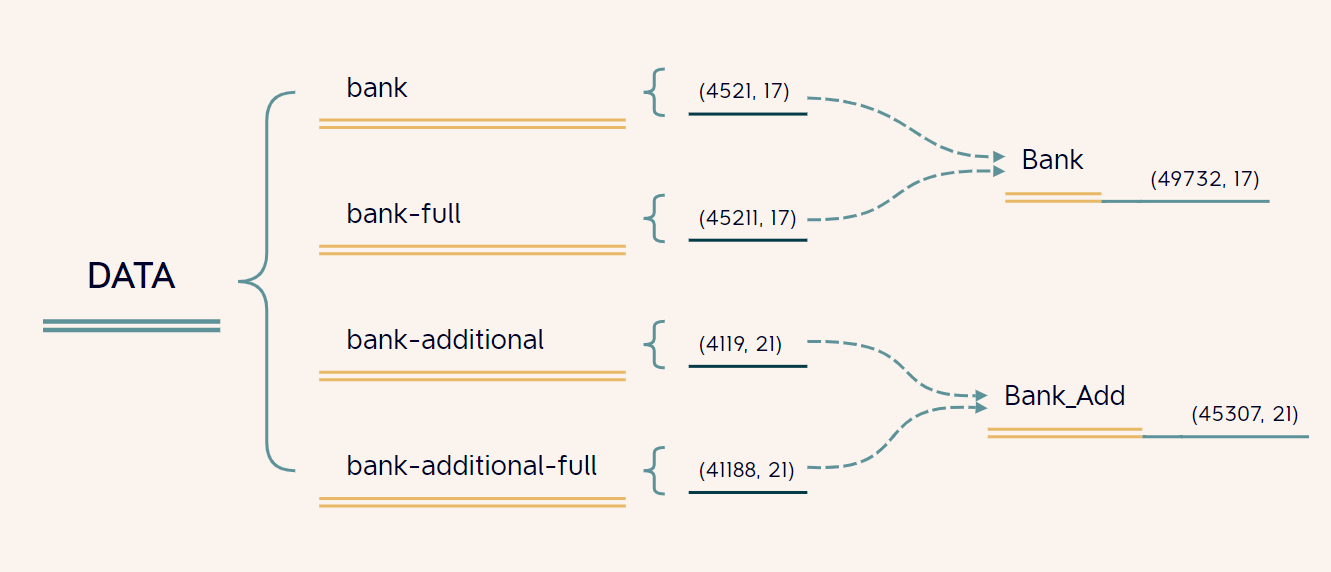
\includegraphics[width=0.8\textwidth]{data/bank_marketing/pic/Data.png}
    \caption{Data Unveiled: Integration and Consolidation of Bank Files}
    \label{fig:data_unveiled}
\end{figure}


\subsection{Attributes and Data Types Overview}
In the analysis of our dataset, we have identified two distinct files, each possessing a unique set of attributes. While some attributes are shared between the two files, there are also attributes that are exclusive to each file. This divergence in attribute composition adds a layer of complexity to our data exploration.

\textbf{File 1 Attributes:}
File 1 exhibits a concise attribute structure, comprising two primary data types: \texttt{int64} and \texttt{object}. This streamlined approach simplifies the data representation, fostering clarity and ease of interpretation.

\textbf{File 2 Attributes:}
Contrastingly, File 2 introduces an additional data type, \texttt{float64}, alongside the common \texttt{int64} and \texttt{object} data types. This expansion in data types implies a more diverse range of information, potentially offering a nuanced perspective on the dataset.

Understanding the nature and distribution of these attributes in each file is pivotal for a comprehensive analysis. It not only enables us to leverage the shared attributes for integrated insights but also allows us to appreciate the unique aspects introduced by the exclusive attributes in each file.

This attribute differentiation sets the stage for a meticulous exploration of the dataset, providing an opportunity to leverage the varied information embedded within File 2 while maintaining a coherent understanding of the attributes shared between the two files.

\begin{figure}[h]
    \centering
    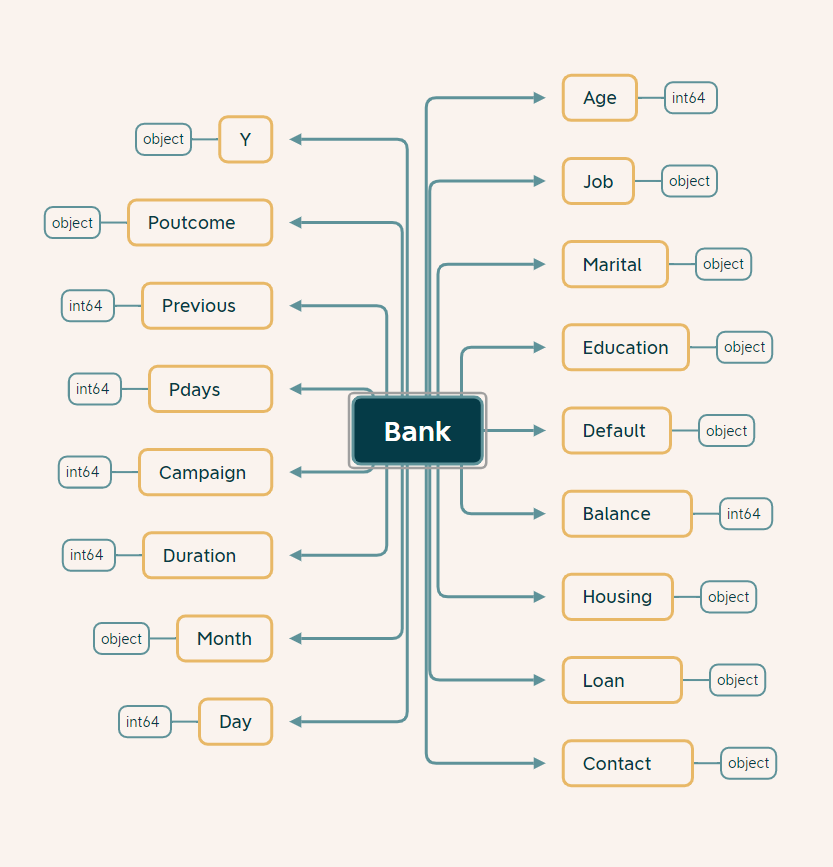
\includegraphics[width=0.4\linewidth]{data/bank_marketing/pic/Bank_attributes .png}\hfill
    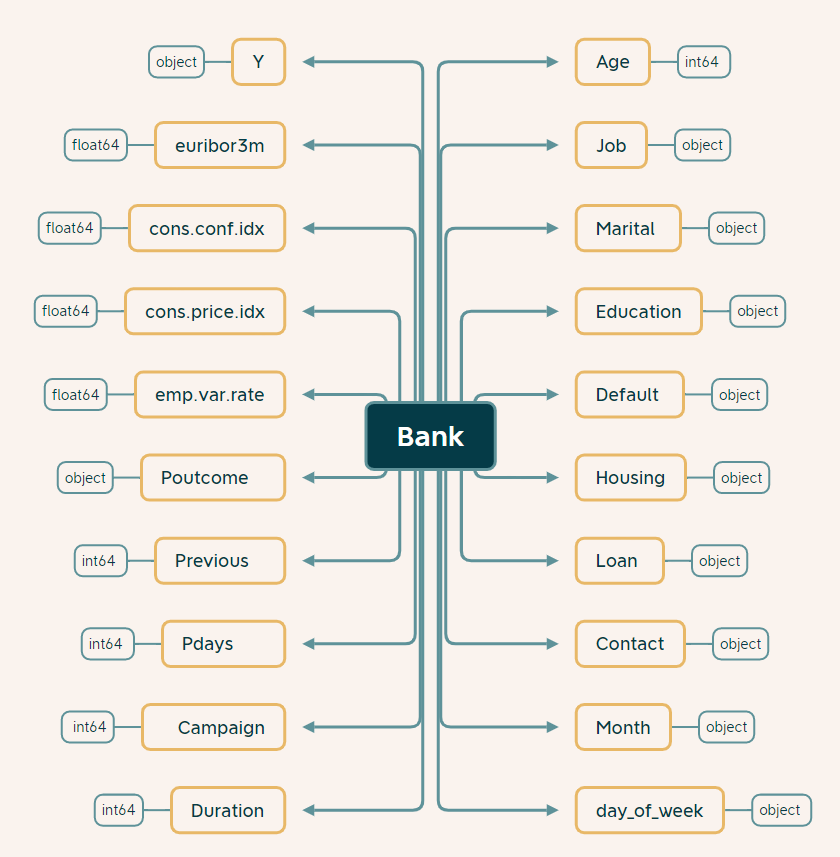
\includegraphics[width=0.4\linewidth]{data/bank_marketing/pic/Bank_Add_attributes .png}
    \caption{Data Attribute Comparison Across Two Files}
    \label{fig:both}
  \end{figure}

  \subsection{Detection of Missing Values}
Missing values are a common challenge in data analysis, impacting the reliability and validity of our findings. This chapter delves into the process of detecting and handling missing values in the datasets: \textit{Bank} and \textit{Bank\_Add}.

An essential aspect of data preprocessing is the identification and handling of missing values. We employed the \textit{msno} library to visualize and analyze missing values in both datasets.

\subsubsection{Detection of Missing Values (File: Bank)}
Upon employing \texttt{msno.matrix} and examining summary statistics, we are pleased to report that no missing values were detected in the \textit{Bank} dataset. This high level of completeness instills confidence in the dataset's integrity.
\begin{figure}[h]
    \centering
    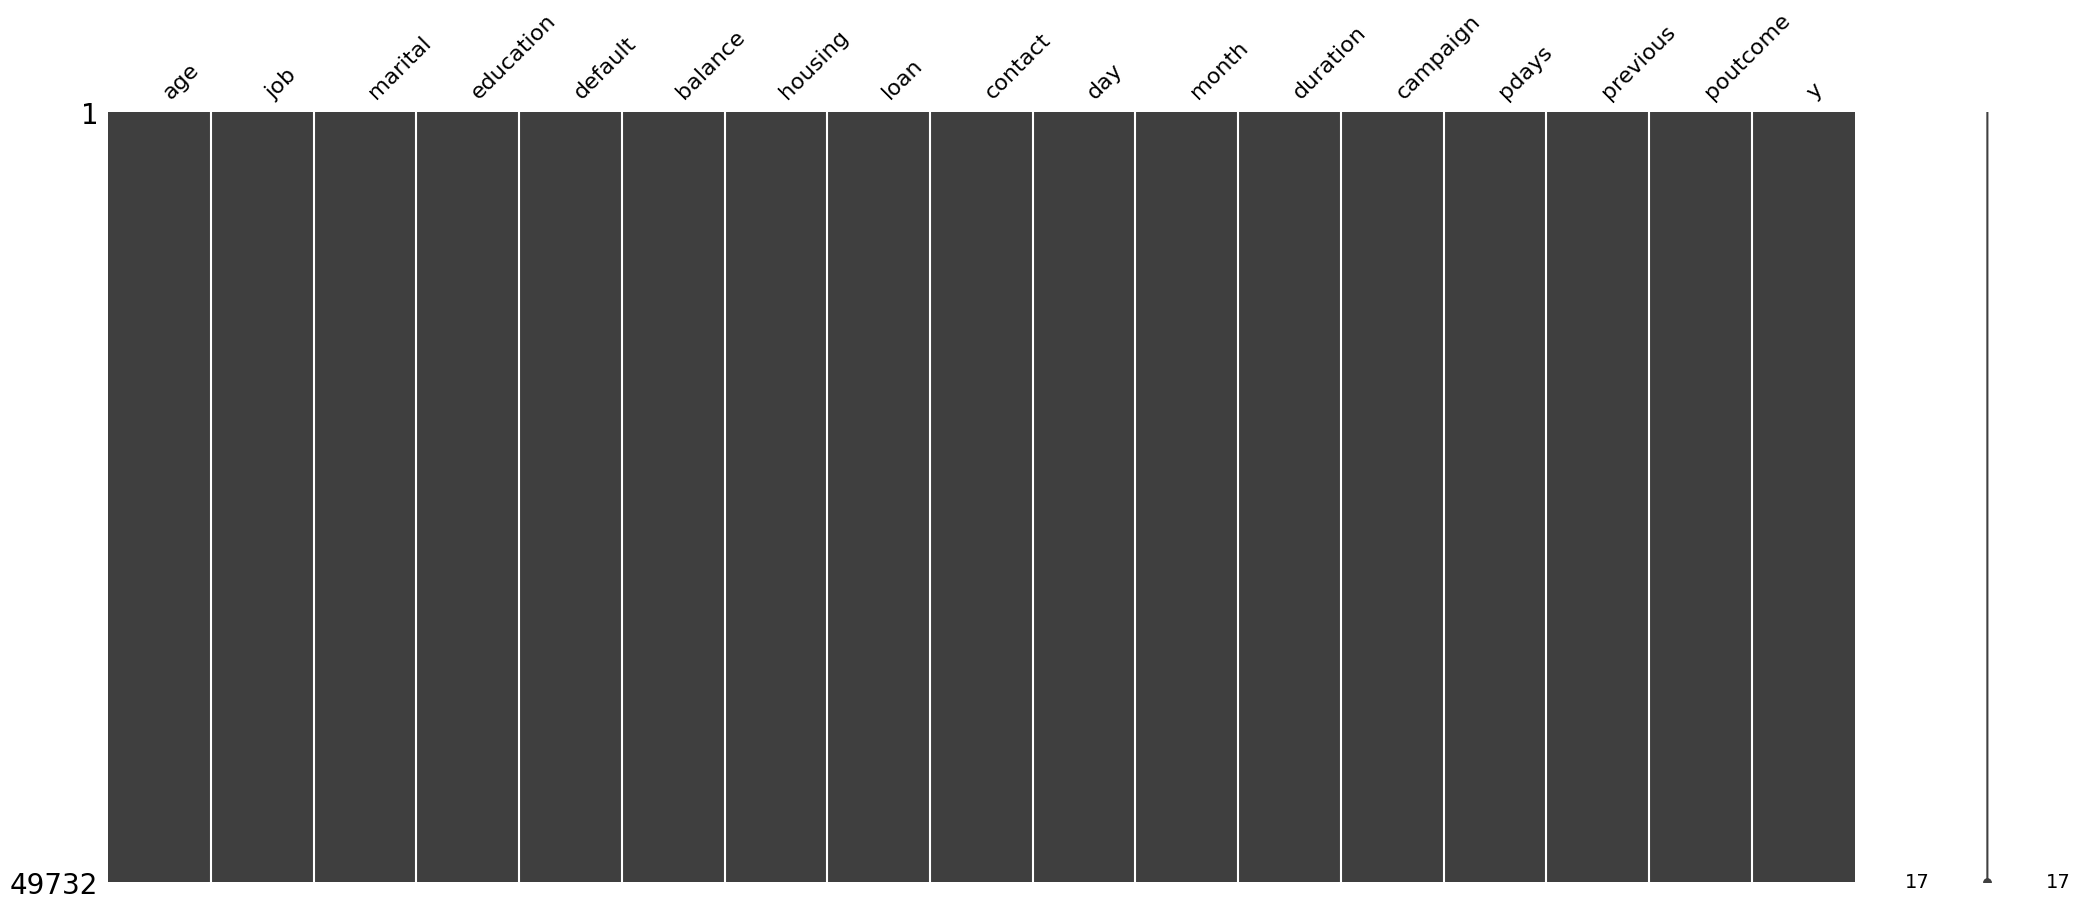
\includegraphics[width=0.8\textwidth]{data/bank_marketing/pic/Outlier/miss_bank.png}
    \caption{Detection of Missing Values in Bank dataset}
    \label{fig:data_unveiled_bank}
\end{figure}

\subsubsection{Detection of Missing Values (File: Bank\_Add)}
Similar to the \textit{Bank} dataset, our analysis of the \textit{Bank\_Add} dataset using \texttt{msno.matrix} revealed no missing values. The dataset is complete across all variables, providing a solid foundation for subsequent analyses.
\begin{figure}[h]
    \centering
    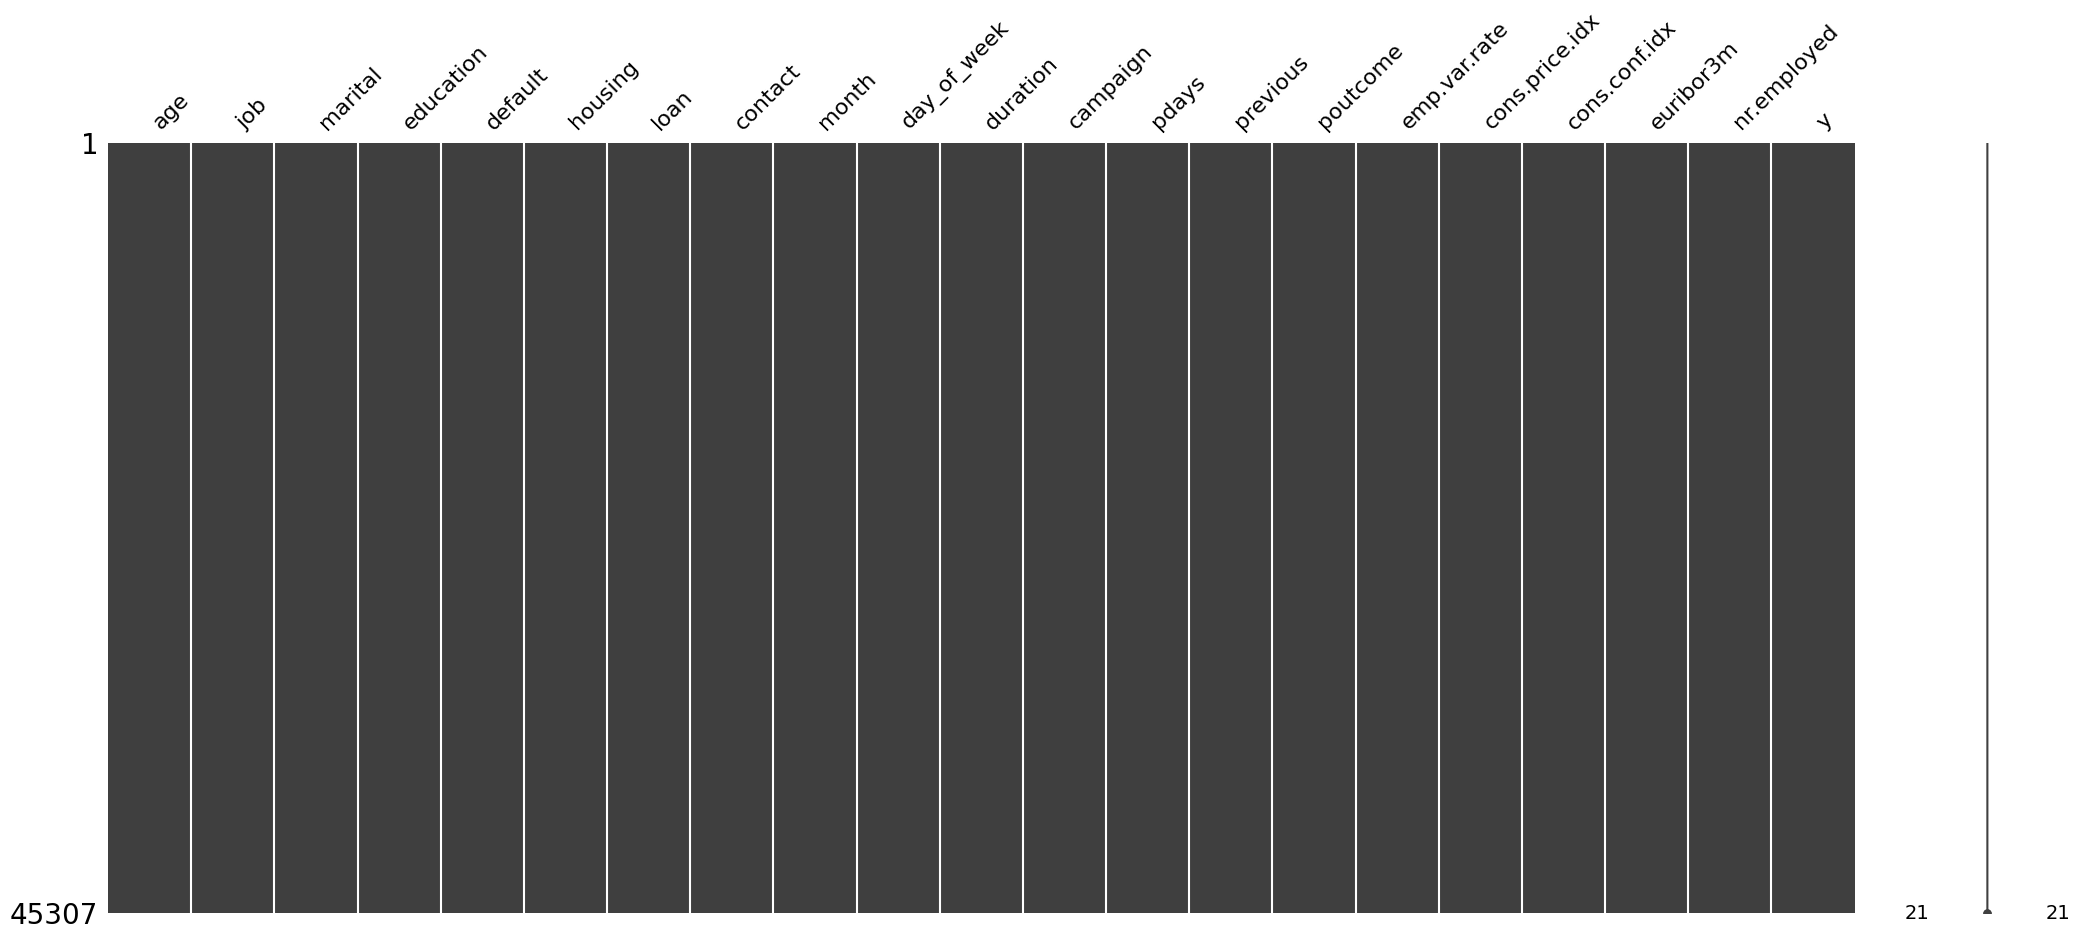
\includegraphics[width=0.8\textwidth]{data/bank_marketing/pic/Outlier/miss_add.png}
    \caption{Detection of Missing Values in Bank\_Add dataset}
    \label{fig:data_unveiled_add}
\end{figure}

The absence of missing values in both the \textit{Bank} and \textit{Bank\_Add} datasets is a positive outcome for our data analysis. This ensures that our subsequent analyses are based on complete and reliable datasets, minimizing the risk of bias introduced by missing information.


\subsection{Statistical Overview: Descriptive Analysis of Key Attributes}
The dataset is comprised of two distinct files: \textit{Bank} and \textit{Bank\_Add}. Let's delve into a detailed exploration of their attributes.

\subsubsection{Summary Statistics for Numeric Attributes (File: Bank)}

The dataset for \textit{Bank} comprises 49,732 entries with 17 columns. The numeric attributes and their summary statistics are as follows:\\  \\

\begin{longtable}{|p{0.15\textwidth}|p{0.4\textwidth}|p{0.45\textwidth}|}
    \caption{Statistics and Distributions}\label{tab:stats}\\
    \hline
    \textbf{Variable} & \textbf{Statistics} & \textbf{Distribution} \\
    \hline
    \endfirsthead
    \multicolumn{3}{c}%
    {\tablename\ \thetable\ -- \textit{Continued from previous page}} \\
    \hline
    \textbf{Variable} & \textbf{Statistics} & \textbf{Distribution} \\
    \hline
    \endhead
    \hline \multicolumn{3}{r}{\textit{Continued on next page}} \\
    \endfoot
    \hline
    \endlastfoot

    Age & 
    \begin{itemize}
        \item Count: 49,732
        \item Mean: 40.96
        \item Standard Deviation: 10.62
        \item Minimum: 18, Maximum: 95
    \end{itemize} & 
    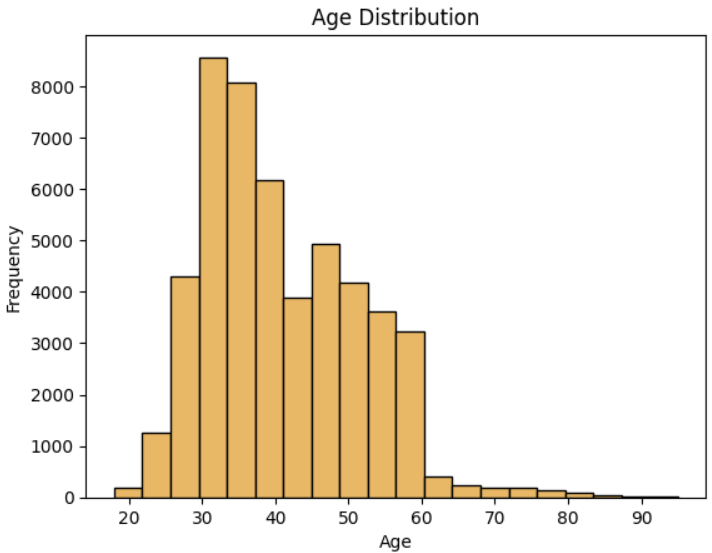
\includegraphics[width=0.45\textwidth]{data/bank_marketing/pic/Bank_Age.png} \\
    \hline
    Balance & 
    \begin{itemize}
        \item Count: 49,732
        \item Mean: 1367.76
        \item Standard Deviation: 3041.61
        \item Minimum: -8019, Maximum: 102127
    \end{itemize} & 
    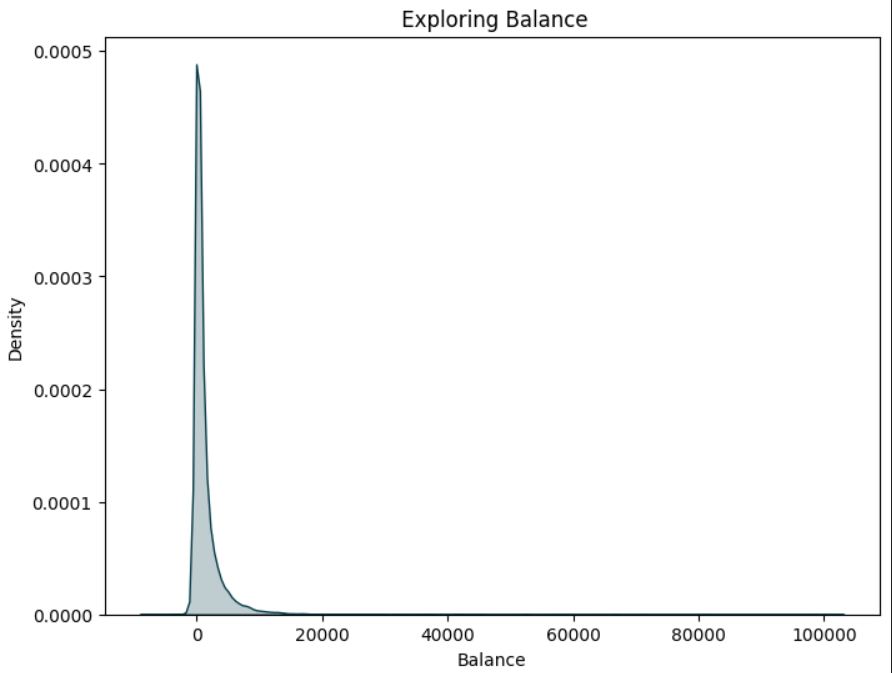
\includegraphics[width=0.45\textwidth]{data/bank_marketing/pic/Bank_balance.png} \\
    \hline
    Day & 
    \begin{itemize}
        \item Count: 49,732
        \item Mean: 15.82
        \item Standard Deviation: 8.32
        \item Minimum: 1, Maximum: 31
    \end{itemize} & 
    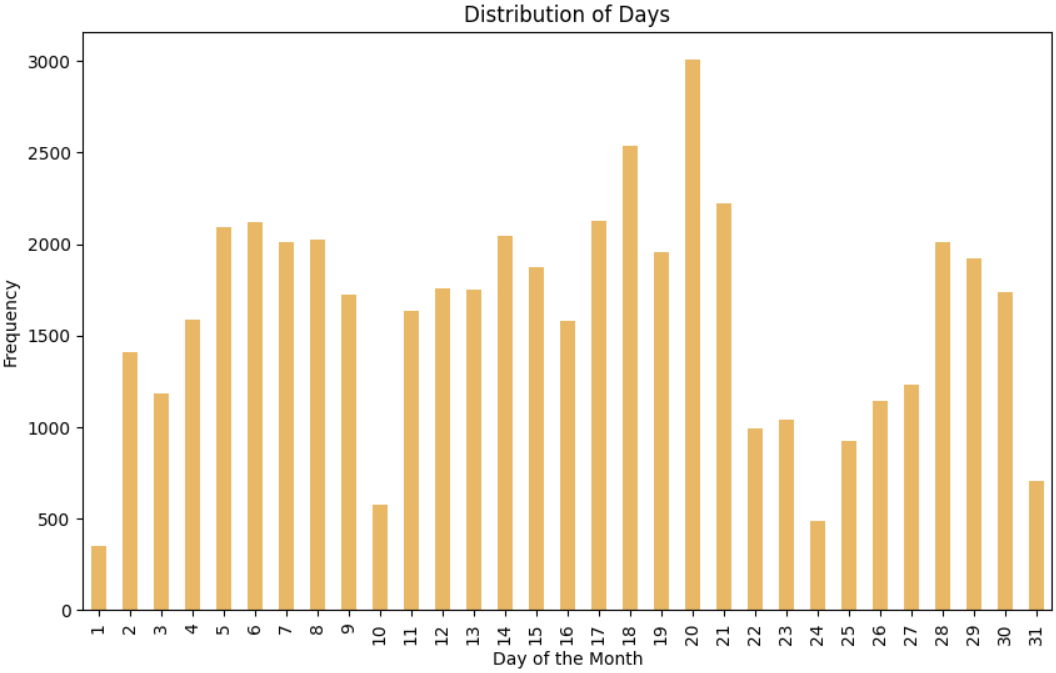
\includegraphics[width=0.45\textwidth]{data/bank_marketing/pic/Bank_day.png} \\
    \hline
    Duration & 
    \begin{itemize}
        \item Count: 49,732
        \item Mean: 258.69
        \item Standard Deviation: 257.74
        \item Minimum: 0, Maximum: 4918
    \end{itemize} & 
    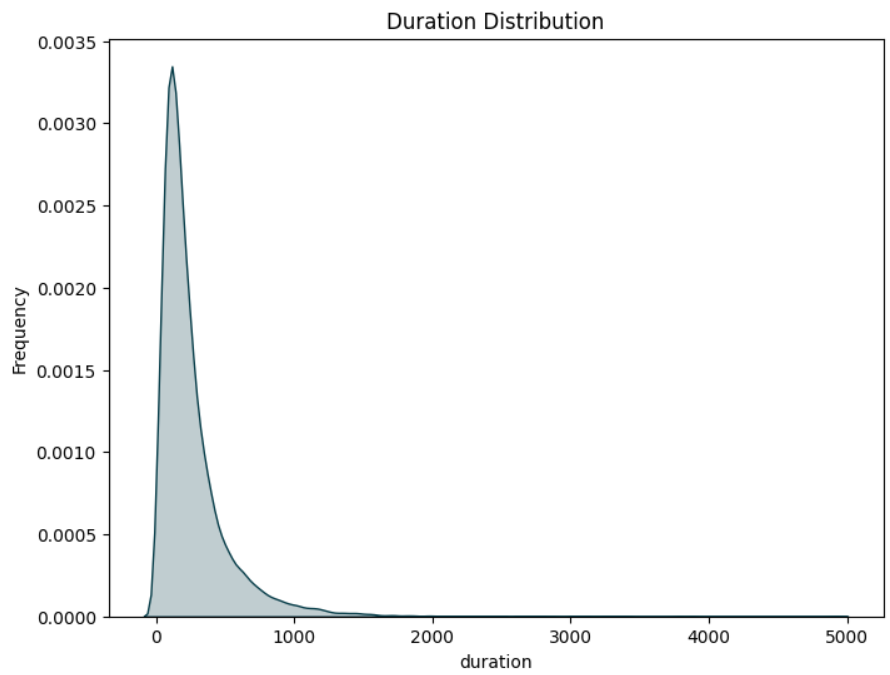
\includegraphics[width=0.45\textwidth]{data/bank_marketing/pic/Bank_duration.png} \\
    \hline
    Campaign & 
    \begin{itemize}
        \item Count: 49,732
        \item Mean: 2.77
        \item Standard Deviation: 3.10
        \item Minimum: 1, Maximum: 63
    \end{itemize} & 
    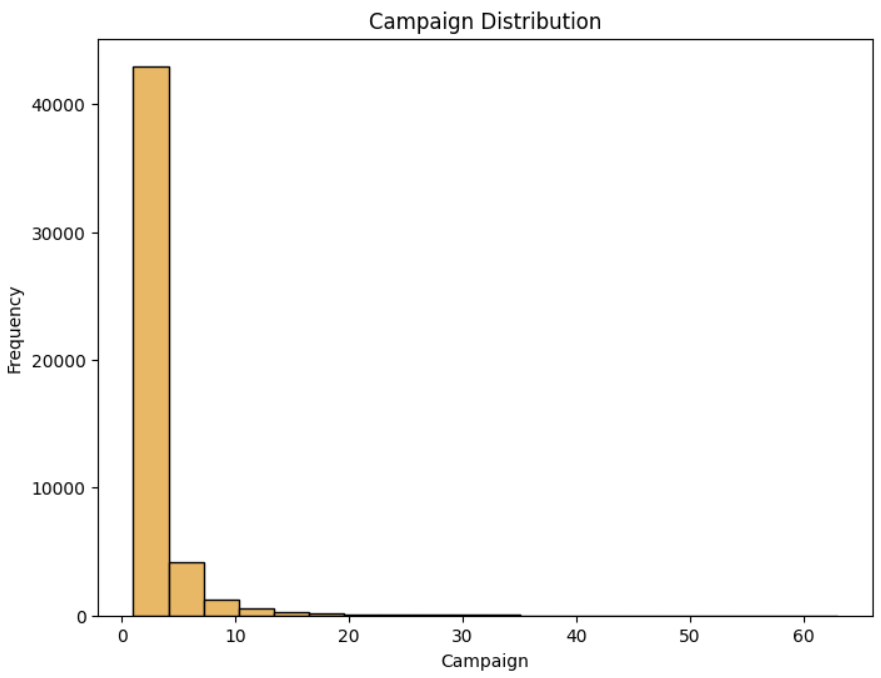
\includegraphics[width=0.45\textwidth]{data/bank_marketing/pic/Bank_campaign.png} \\
    \hline
    Pdays & 
    \begin{itemize}
        \item Count: 49,732
        \item Mean: 40.16
        \item Standard Deviation: 100.13
        \item Minimum: -1, Maximum: 871
    \end{itemize} & 
    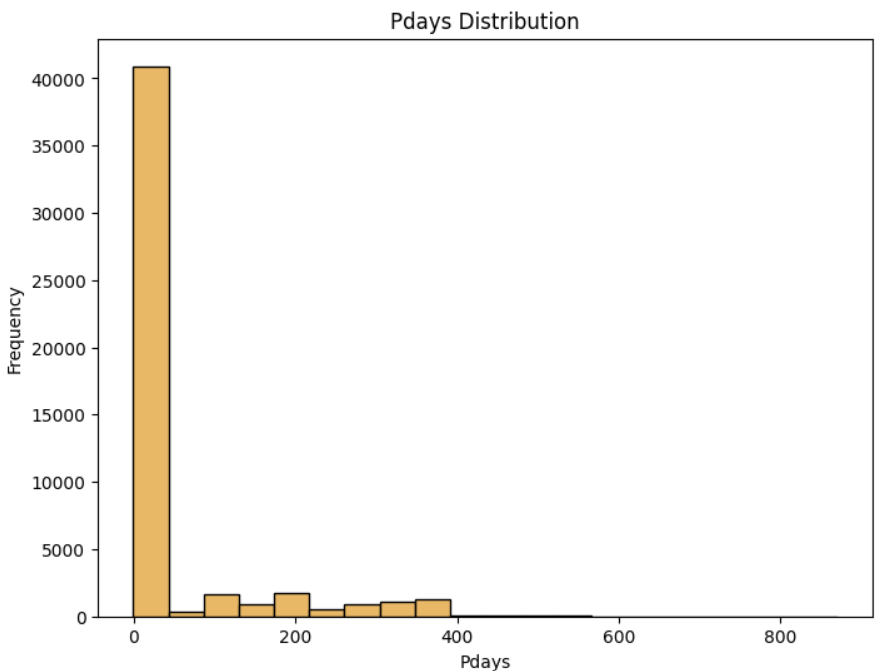
\includegraphics[width=0.45\textwidth]{data/bank_marketing/pic/Bank_pdays.png} \\
    \hline
    Previous & 
    \begin{itemize}
        \item Count: 49,732
        \item Mean: 0.58
        \item Standard Deviation: 2.25
        \item Minimum: 0, Maximum: 275
    \end{itemize} & 
    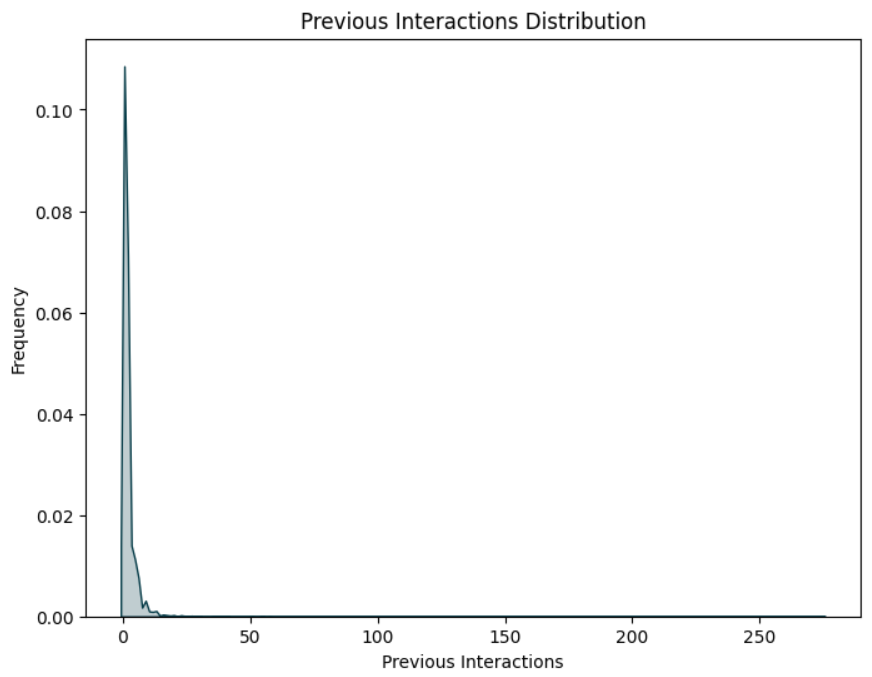
\includegraphics[width=0.45\textwidth]{data/bank_marketing/pic/Bank_Previous.png} \\
    \hline
\end{longtable}

\subsubsection{Summary Statistics for Numeric Attributes (File: Bank\_Add)}

The dataset for \textit{Bank\_Add} consists of 45,307 entries with 21 columns. The numeric attributes and their summary statistics are as follows:\\ \\

\begin{longtable}{|p{0.15\textwidth}|p{0.4\textwidth}|p{0.45\textwidth}|}
    \caption{Statistics and Distributions}\label{tab:stats}\\
    \hline
    \textbf{Variable} & \textbf{Statistics} & \textbf{Distribution} \\
    \hline
    \endfirsthead
    \multicolumn{3}{c}%
    {\tablename\ \thetable\ -- \textit{Continued from previous page}} \\
    \hline
    \textbf{Variable} & \textbf{Statistics} & \textbf{Distribution} \\
    \hline
    \endhead
    \hline \multicolumn{3}{r}{\textit{Continued on next page}} \\
    \endfoot
    \hline
    \endlastfoot

    Age & 
    \begin{itemize}
        \item Count: 45,307
        \item Mean: 40.03
        \item Standard Deviation: 10.41
        \item Minimum: 17, Maximum: 98
    \end{itemize} & 
    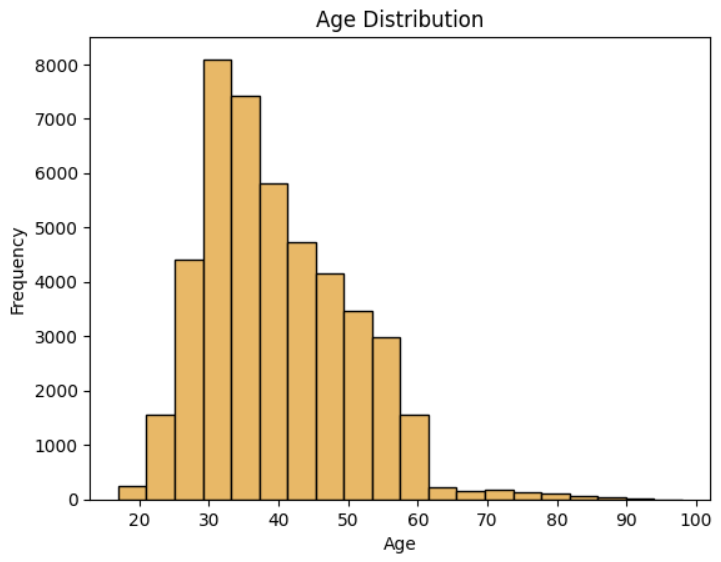
\includegraphics[width=0.45\textwidth]{data/bank_marketing/pic/Bank_Add_Age.png} \\
    \hline
    Duration & 
    \begin{itemize}
        \item Count: 45,307
        \item Mean: 258.15
        \item Standard Deviation: 258.86
        \item Minimum: 0, Maximum: 4918
    \end{itemize} & 
    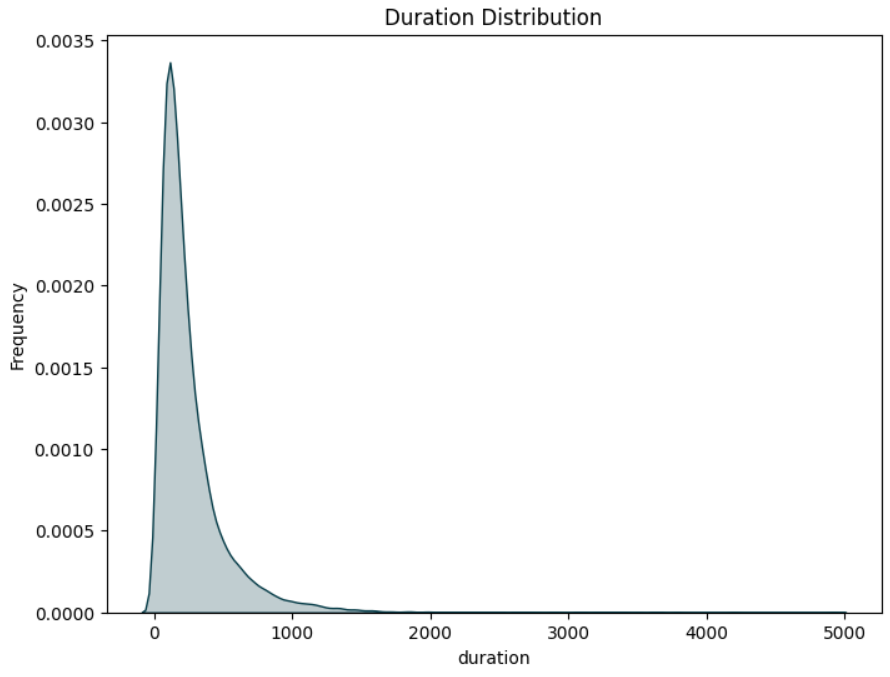
\includegraphics[width=0.45\textwidth]{data/bank_marketing/pic/Bank_Add_duration.png} \\
    \hline
    Campaign & 
    \begin{itemize}
        \item Count: 45,307
        \item Mean: 2.56
        \item Standard Deviation: 2.75
        \item Minimum: 1, Maximum: 56
    \end{itemize} & 
    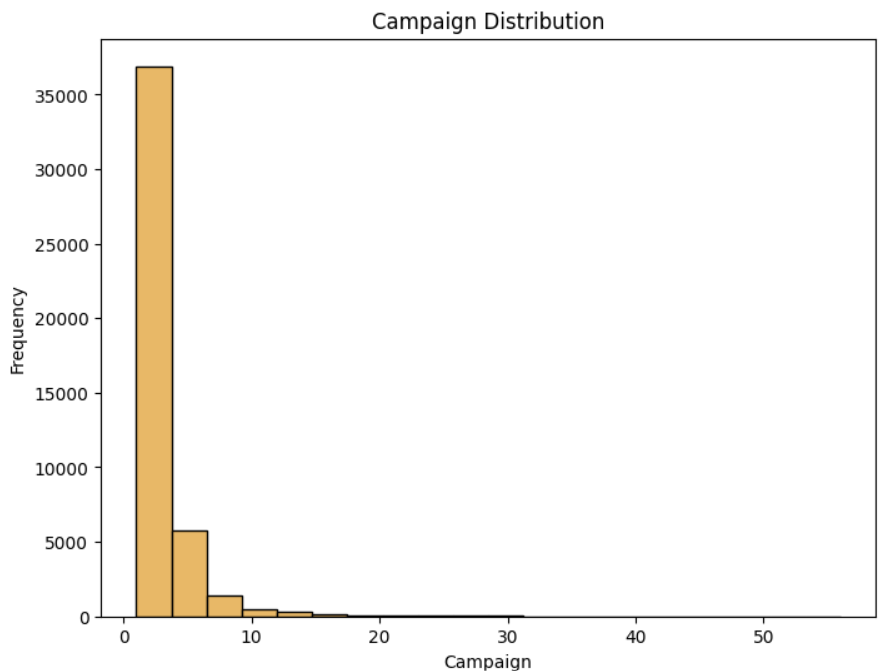
\includegraphics[width=0.45\textwidth]{data/bank_marketing/pic/Bank_Add_campaign.png} \\
    \hline
    Pdays & 
    \begin{itemize}
        \item Count: 45,307
        \item Mean: 962.29
        \item Standard Deviation: 187.37
        \item Minimum: 0, Maximum: 999
    \end{itemize} & 
    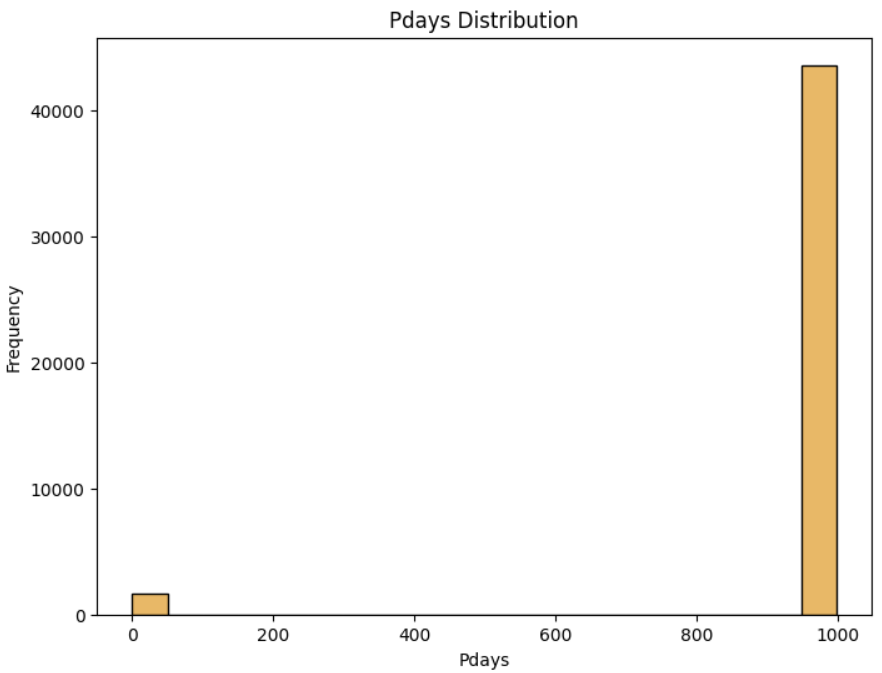
\includegraphics[width=0.45\textwidth]{data/bank_marketing/pic/Bank_Add_pdays.png} \\
    \hline
    Previous & 
    \begin{itemize}
        \item Count: 45,307
        \item Mean: 0.17
        \item Standard Deviation: 0.50
        \item Minimum: 0, Maximum: 7
    \end{itemize} & 
    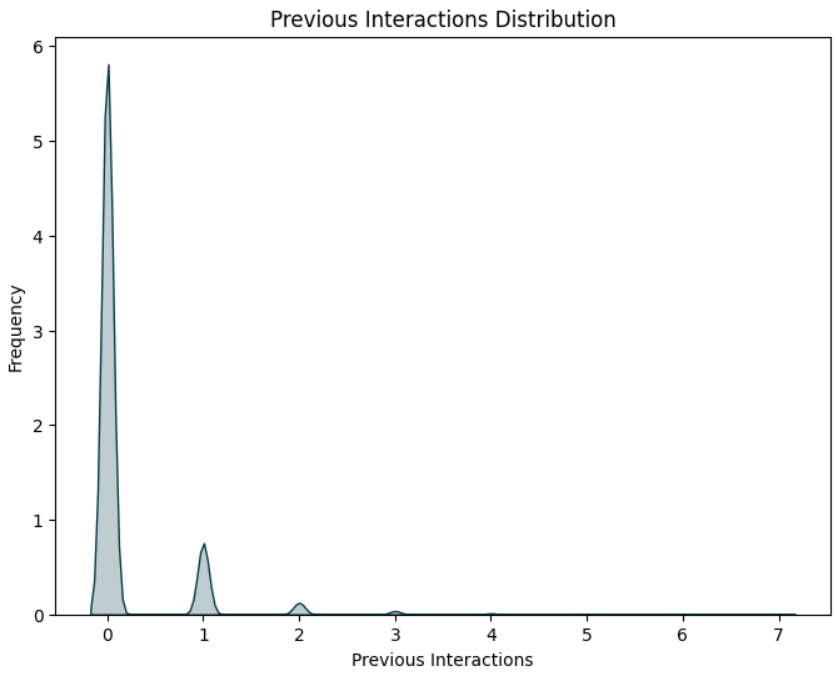
\includegraphics[width=0.45\textwidth]{data/bank_marketing/pic/Bank_Add_Previous.png} \\
    \hline
    Employment Variation Rate & 
    \begin{itemize}
        \item Count: 45,307
        \item Mean: 0.08
        \item Standard Deviation: 1.57
        \item Minimum: -3.4, Maximum: 1.4
    \end{itemize} & 
    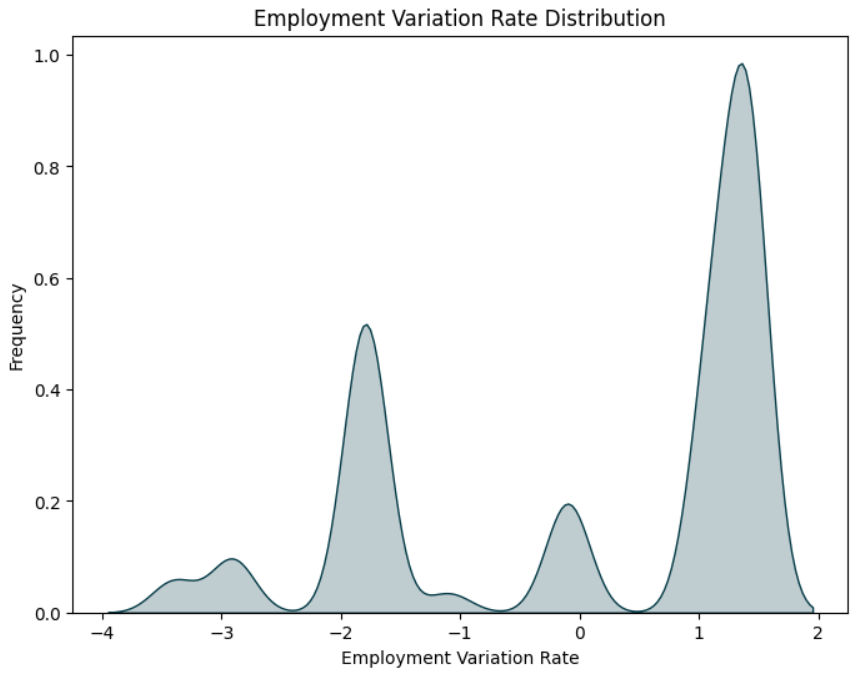
\includegraphics[width=0.45\textwidth]{data/bank_marketing/pic/Bank_Add_emp.png} \\
    \hline
    Consumer Price Index & 
    \begin{itemize}
        \item Count: 45,307
        \item Mean: 93.58
        \item Standard Deviation: 0.58
        \item Minimum: 92.20, Maximum: 94.77
    \end{itemize} & 
    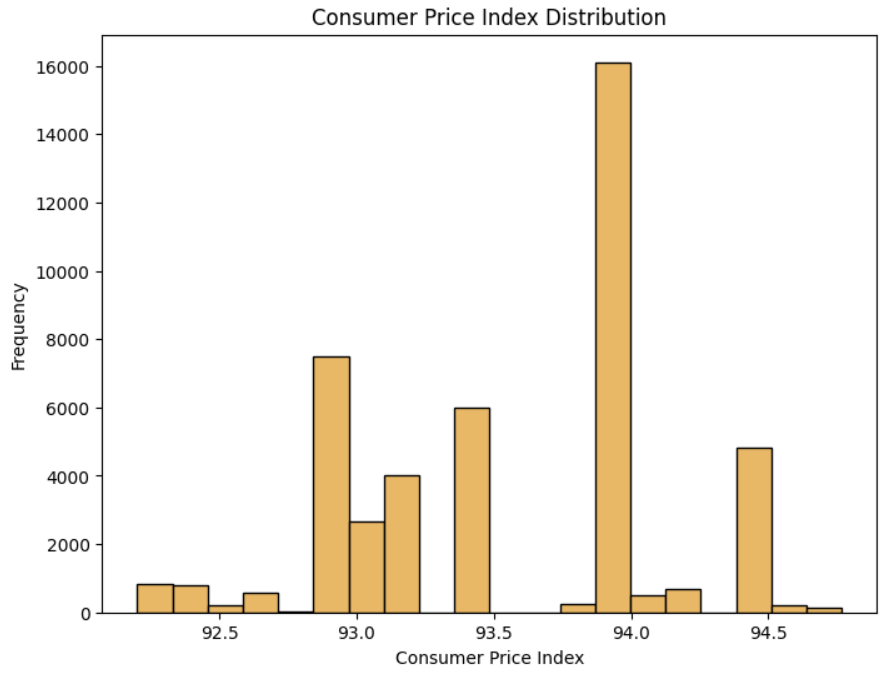
\includegraphics[width=0.45\textwidth]{data/bank_marketing/pic/Bank_Add_cons_price.png} \\
    \hline
    Consumer Confidence Index & 
    \begin{itemize}
        \item Count: 45,307
        \item Mean: -40.50
        \item Standard Deviation: 4.63
        \item Minimum: -50.80, Maximum: -26.90
    \end{itemize} & 
    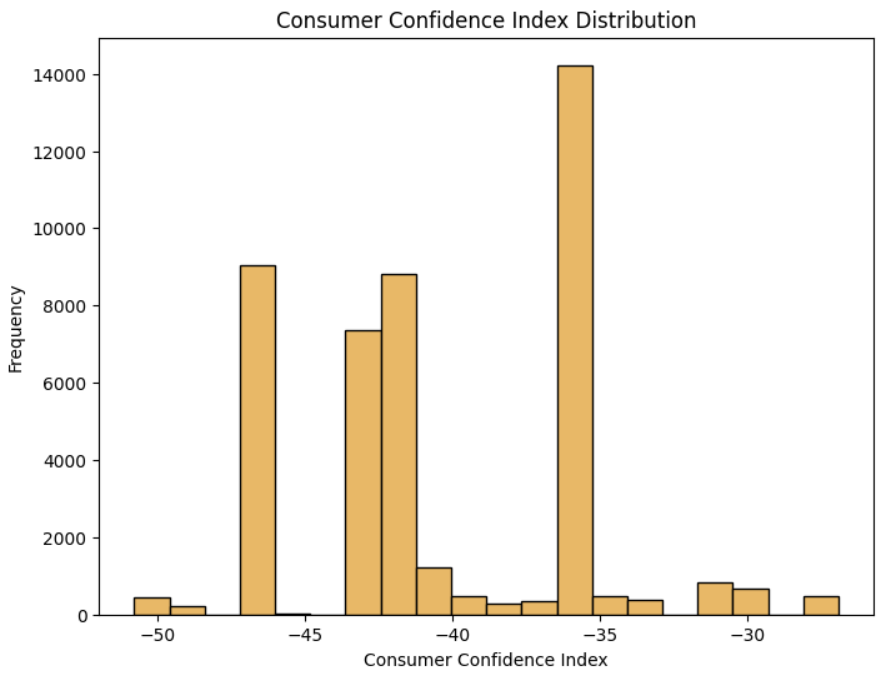
\includegraphics[width=0.45\textwidth]{data/bank_marketing/pic/Bank_Add_cons_conf.png} \\
    \hline
    EURIBOR 3-Month Rate & 
    \begin{itemize}
        \item Count: 45,307
        \item Mean: 3.62
        \item Standard Deviation: 1.73
        \item Minimum: 0.63, Maximum: 5.05
    \end{itemize} & 
    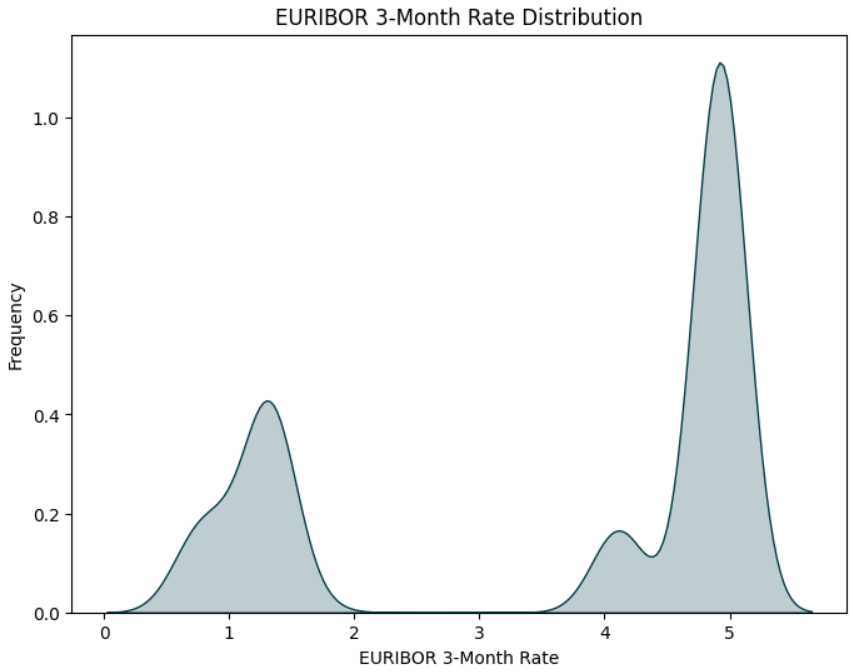
\includegraphics[width=0.45\textwidth]{data/bank_marketing/pic/Bank_Add_eur.png} \\
    \hline
    Number of Employees & 
    \begin{itemize}
        \item Count: 45,307
        \item Mean: 5166.99
        \item Standard Deviation: 72.38
        \item Minimum: 4963.60, Maximum: 5228.10
    \end{itemize} & 
    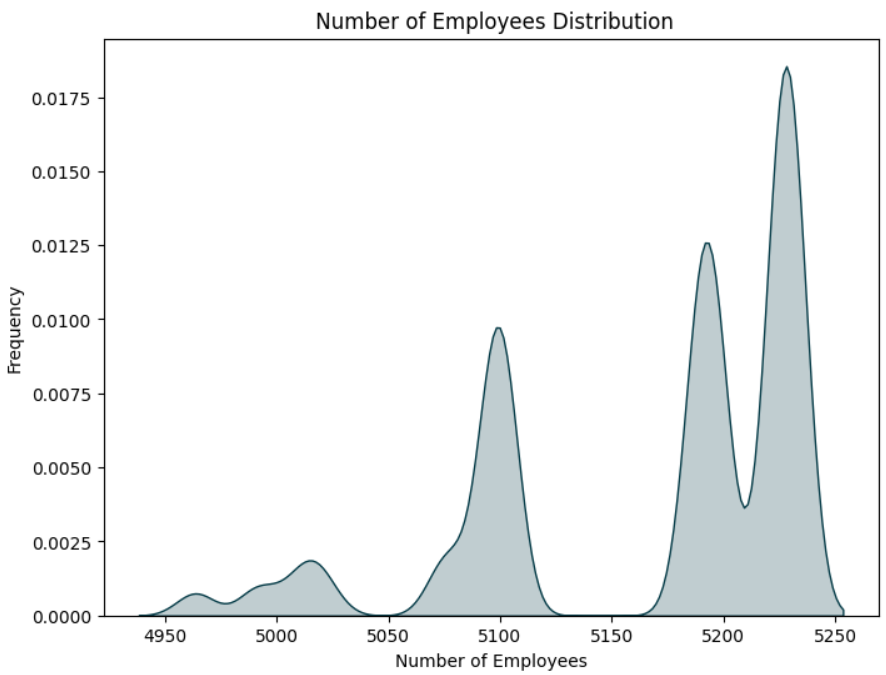
\includegraphics[width=0.45\textwidth]{data/bank_marketing/pic/Bank_Add_nr.png} \\
    \hline
\end{longtable}

In summary, this comprehensive overview provides essential insights into the distribution and characteristics of key attributes in both datasets. These findings lay the foundation for further in-depth analyses and model building.
\\ \\ \\ \\ \\


\subsection{Correlation Analysis of Numerical Variables}
In this section, we conduct exploratory data analysis on two datasets: \textit{Bank} and \textit{Bank\_Add}. We employ heatmaps and pair plots to unveil patterns, correlations, and relationships within each dataset.


 \subsubsection{Correlation Heatmap (File: Bank)}
 
 The correlation heatmap for the \textit{Bank} dataset (Figure \ref{fig:heatmap_bank}) visualizes the relationships between numerical variables. Key observations include:
 \\

 \begin{figure}[h]
                \centering
                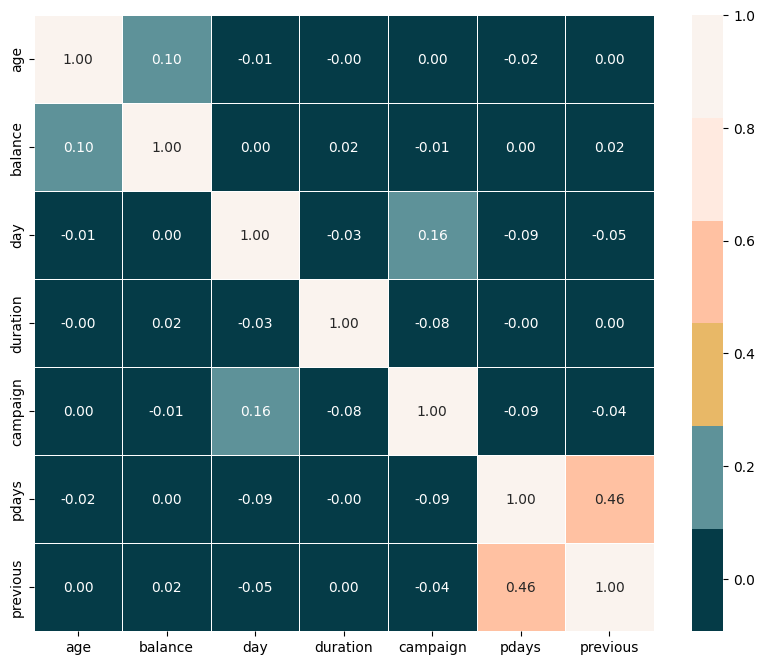
\includegraphics[width=0.4\textwidth]{data/bank_marketing/pic/Bank_Corr.png}
                \caption{Correlation Heatmap}
                \label{fig:heatmap_bank}
            \end{figure}
\begin{itemize}
    \item Bright shades, represented by colors such as Sigma Warm Red, indicate stronger correlations.
    \item Positive and negative correlations are discernible.
    \item The heatmap aids in identifying potential multicollinearity among features.
\end{itemize}

 \subsubsection{Multivariate Analysis  (File: Bank)}
 The pair plot for the \textit{Bank} dataset (Figure \ref{fig:pair_plot_bank}) offers insights into the interactions between numerical variables.
 \begin{figure}[h]
                \centering
                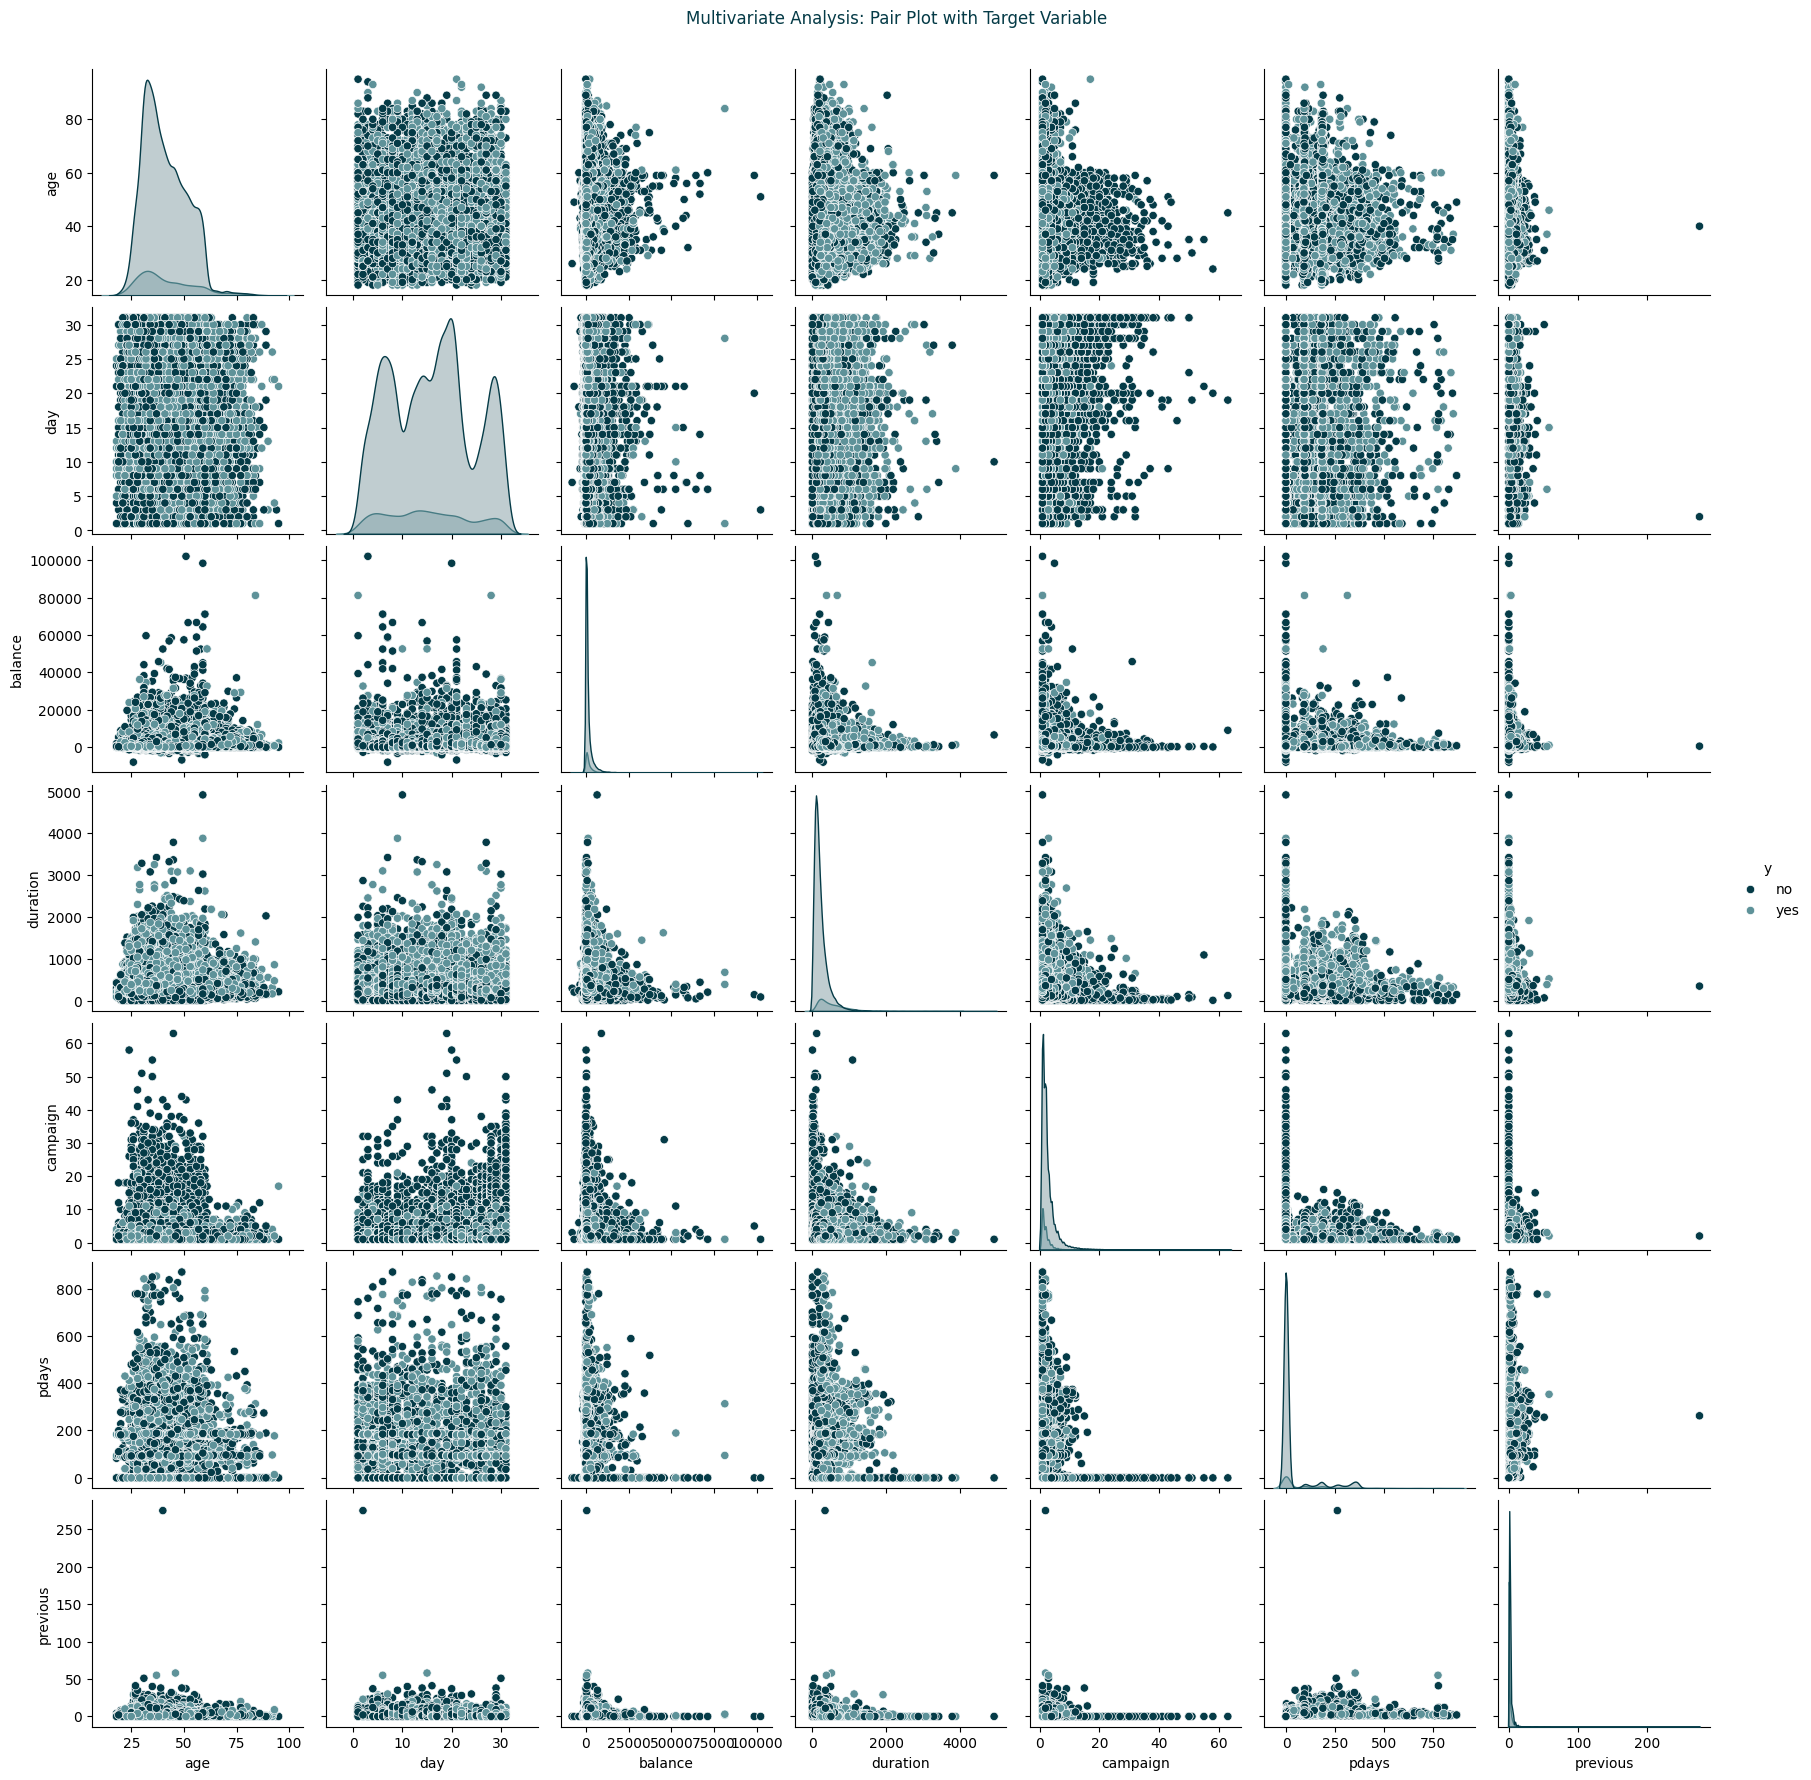
\includegraphics[width=0.6\textwidth]{data/bank_marketing/pic/Bank_pairplot.png}
                \caption{Multivariate Analysis}
                \label{fig:pair_plot_bank}
            \end{figure}
\begin{itemize}
    \item Scatterplots reveal patterns and potential relationships.
    \item Differentiation by the target variable ("y") provides context for variable distributions.
    \vspace{300pt}
\end{itemize}


\subsubsection{Correlation Heatmap (File: Bank\_Add)}
The correlation heatmap for the \textit{Bank\_Add} dataset (Figure \ref{fig:heatmap_bank_add}) showcases correlations among numerical variables. Key insights include:
\begin{figure}[h]
                \centering
                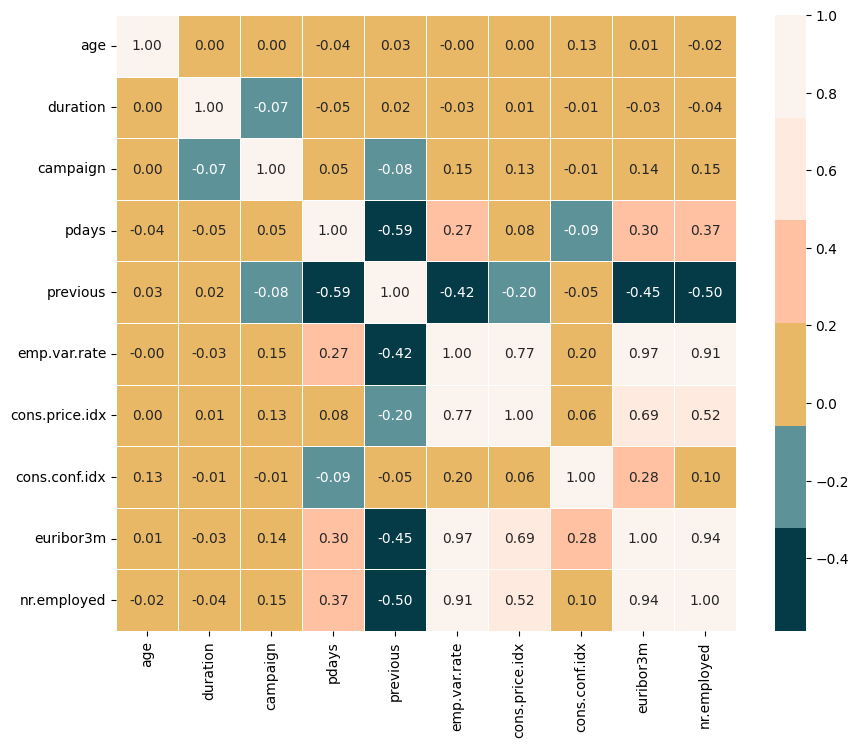
\includegraphics[width=0.7\textwidth]{data/bank_marketing/pic/Bank_Add_Corr.png}
                \caption{Correlation Heatmap}
                \label{fig:heatmap_bank_add}
            \end{figure}
        \begin{itemize}
            \item Similar to \textit{Bank}, bright shades, such as Sigma Warm Red, indicate varying degrees of correlation.
            \item Patterns specific to this dataset aid in understanding feature relationships
            \vspace{300pt}
        \end{itemize}

\subsubsection{Multivariate Analysis  (File: Bank\_Add)}
The pair plot for the \textit{Bank\_Add} dataset (Figure \ref{fig:pair_plot_bank_add}) complements the correlation heatmap. Important takeaways are:
             \begin{figure}[h]
                \centering
                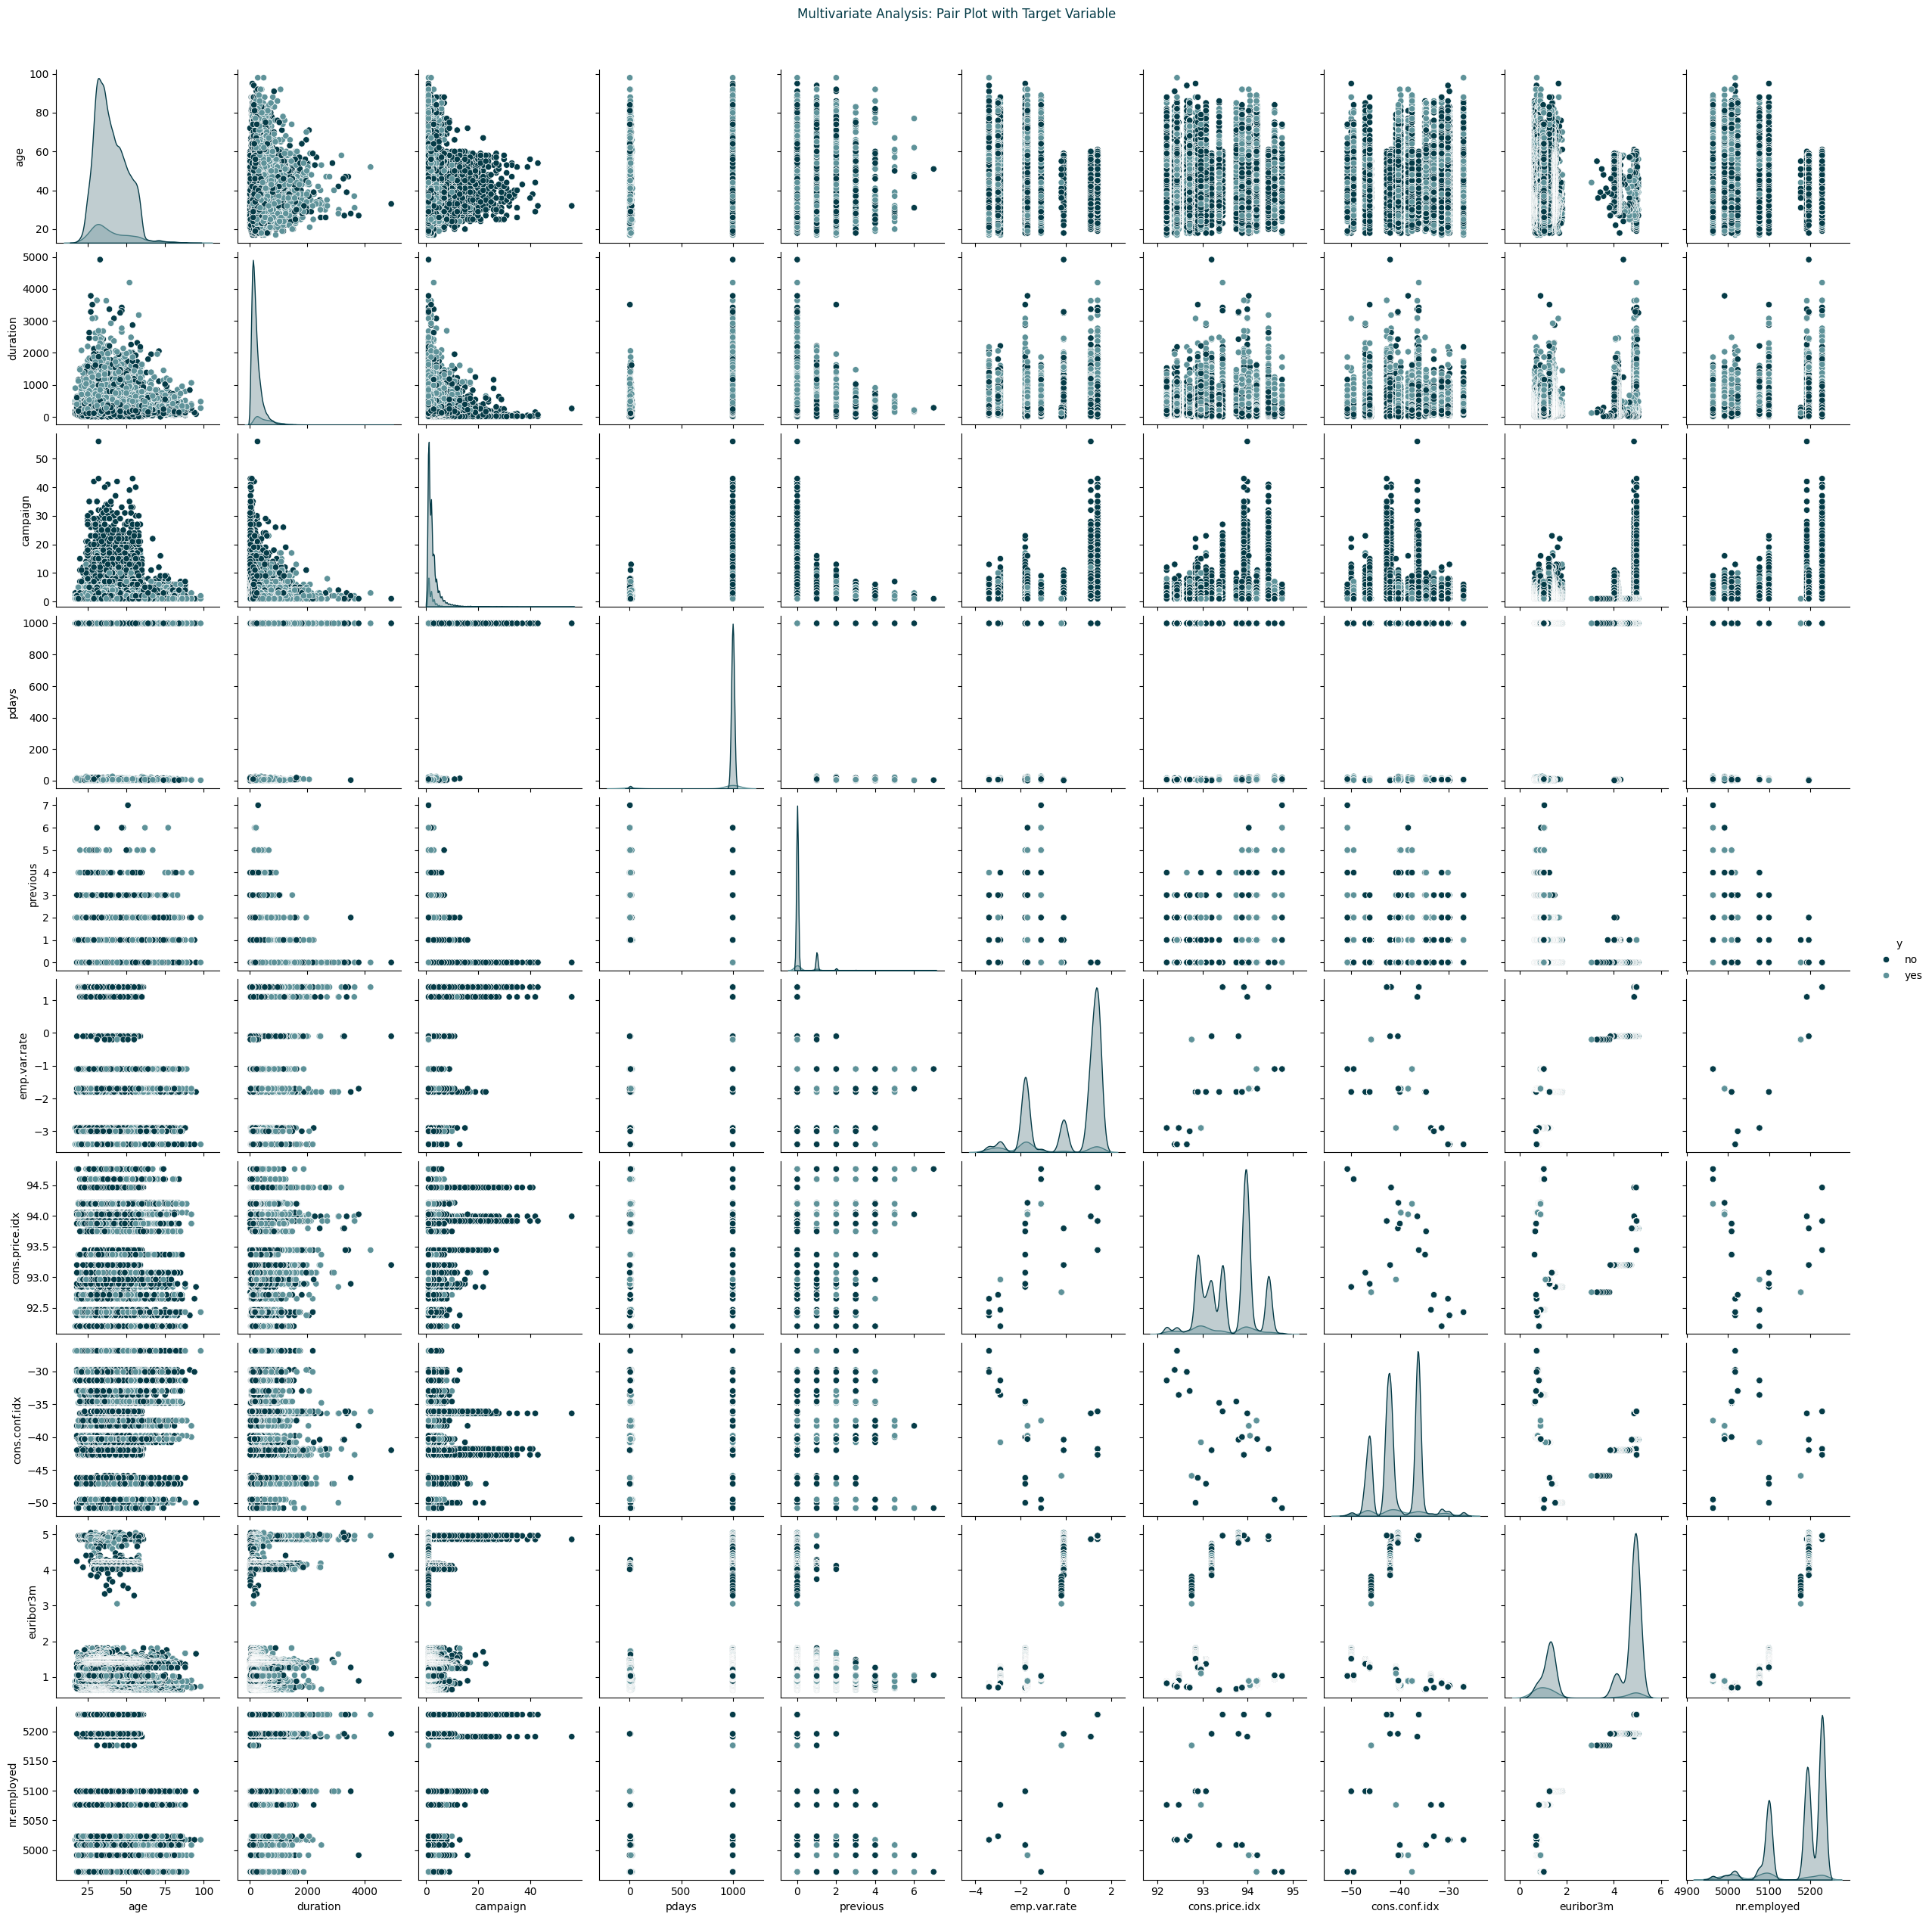
\includegraphics[width=0.9\textwidth]{data/bank_marketing/pic/Bank_Add_pairplot.png}
                \caption{Multivariate Analysis}
                \label{fig:pair_plot_bank_add}
            \end{figure}
            \begin{itemize}
                \item Scatterplots unveil patterns unique to this dataset.
                \item Hue differentiation by the target variable enhances interpretability.
                \vspace{300pt}   
            \end{itemize}

            In conclusion, these exploratory analyses lay the groundwork for further investigations and model development. The revealed patterns and correlations serve as a compass, guiding subsequent steps in the data analysis journey. Future sections will delve deeper into specific aspects, leveraging the knowledge gained from this comprehensive exploration.


            \subsection{Unveiling Categorical Insights}
 
            In this section, we embark on a comprehensive exploration of the categorical variables within our datasets, shedding light on key aspects that influence patterns and trends. Categorical data, representing characteristics such as job roles, marital status, education levels, and more, play a pivotal role in understanding the demographic composition and preferences of the subjects under study.
            Our analysis centers on two datasets: \textit{Bank} and \textit{Bank\_Add}. By scrutinizing the distribution, frequencies, and relationships within these categorical variables, we aim to derive actionable insights that may guide decision-making processes.
            Through a combination of descriptive statistics, visualizations, and interpretative narratives, this section seeks to uncover the nuances encapsulated in the categorical dimensions of our datasets. The exploration not only provides a snapshot of the current state but also serves as a foundation for subsequent analyses, allowing us to delve deeper into the intricacies of the data.
            Join us on this journey as we navigate through the categorical landscape, revealing patterns that contribute to a richer understanding of the subjects at hand.
           
            \subsubsection{Summary of Categorical Variables (File: Bank) }
            The presented table (Table \ref{tab:my_label}) provides a comprehensive summary of key categorical variables within the dataset. Each row corresponds to a specific attribute, such as job type, marital status, education level, default status, housing and loan information, contact method, month of contact, the outcome of the previous marketing campaign (Poutcome), and the target variable 'Y.' The columns offer essential insights into the distribution, variety, and prevalence of these attributes. 
            \begin{table}[h]
               \centering
               \begin{tabular}{lcccc}
                   \textbf{Attributes} & \textbf{Count} & \textbf{Unique} & \textbf{Top} & \textbf{Freq} \\
                   \hline
                   Job & 49732 & 12 & \textit{blue-collar} & 10678 \\ 
                   Marital & 49732 & 3 & \textit{married} & 30011 \\ 
                   Education & 49732 & 4 & \textit{secondary} & 25508 \\ 
                   Default & 49732 & 2 & \textit{no} & 48841 \\
                   Housing & 49732 & 2 & \textit{yes} & 27689 \\
                   Loan & 49732 & 2 & \textit{no} & 41797 \\
                   Contact & 49732 & 3 & \textit{cellular} & 32181 \\
                   Month & 49732 & 12 & \textit{May} & 15164 \\
                   Poutcome & 49732 & 4 & \textit{unknown} & 40664 \\
                   Y & 49732 & 2 & \textit{no }& 43922 \\
               \end{tabular}
               \caption{Summary Statistics of Categorical Variables in the Dataset.}
               \label{tab:my_label}
           \end{table}
           
           \begin{longtable}{|l|c|}
               \hline
               \textbf{Attributes} & \textbf{Distribution Visualization} \\
               \hline
               \endhead
               Job & 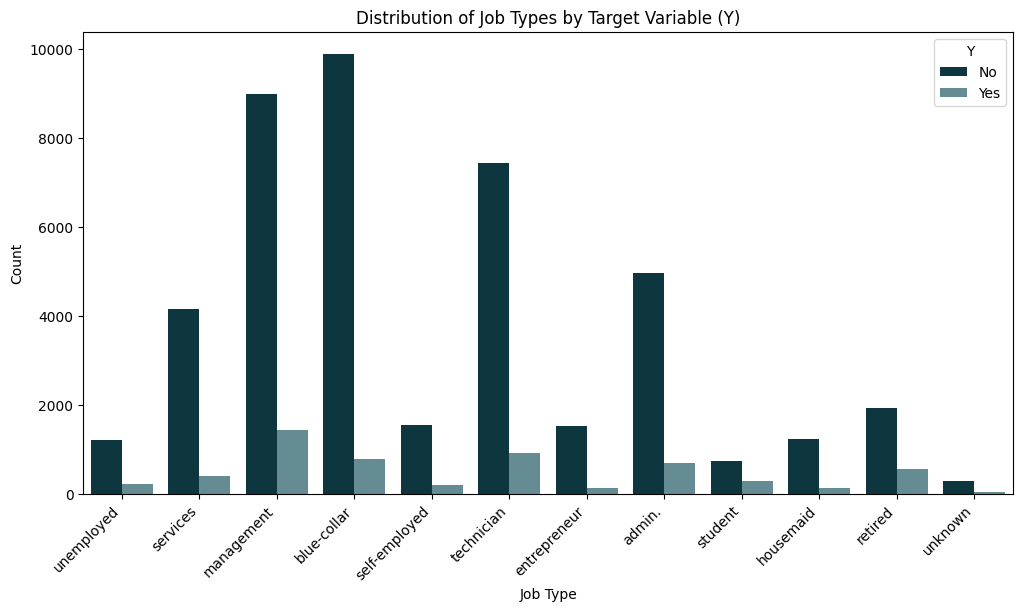
\includegraphics[width=0.7\linewidth]{data/bank_marketing/pic/Bank_job.png} \\ \hline
               Marital & 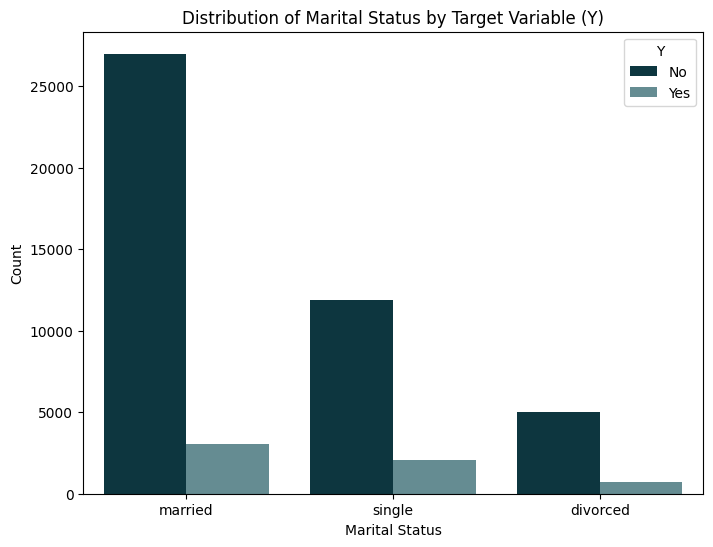
\includegraphics[width=0.7\linewidth]{data/bank_marketing/pic/Bank_marital.png} \\ \hline
               Education & 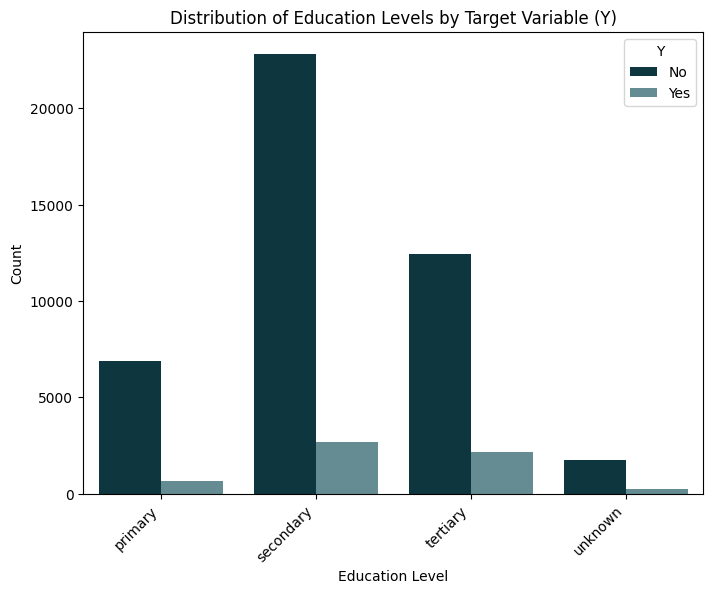
\includegraphics[width=0.7\linewidth]{data/bank_marketing/pic/Bank_edu.png} \\ \hline
               Default & 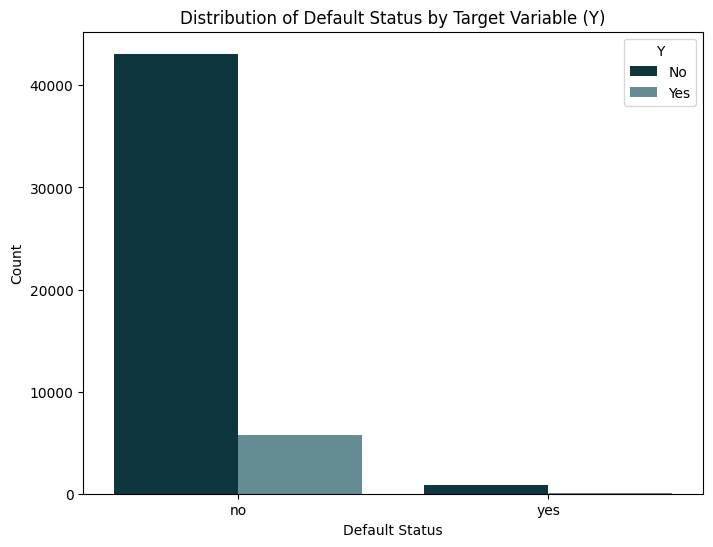
\includegraphics[width=0.7\linewidth]{data/bank_marketing/pic/Bank_def.png} \\ \hline 
               Housing & 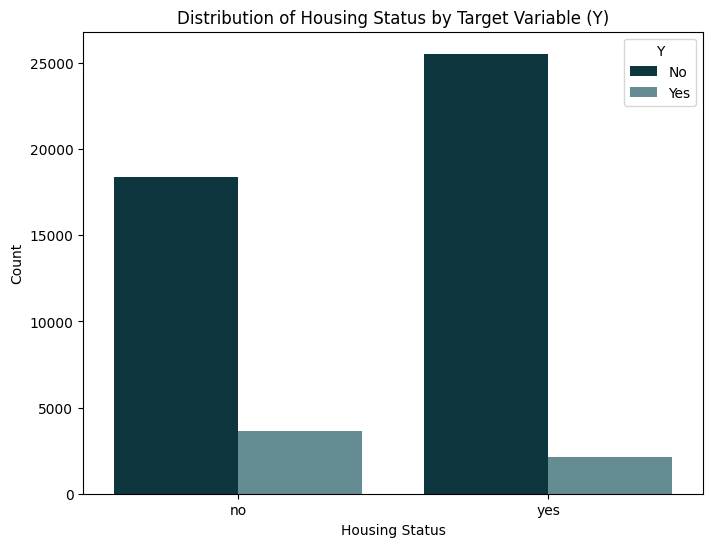
\includegraphics[width=0.7\linewidth]{data/bank_marketing/pic/Bank_Hous.png} \\ \hline
               Loan & 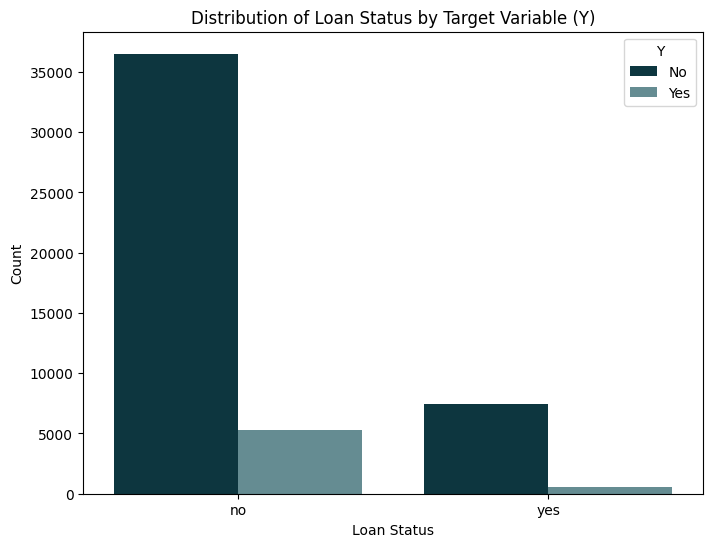
\includegraphics[width=0.7\linewidth]{data/bank_marketing/pic/Bank_loan.png} \\ \hline 
               Contact & 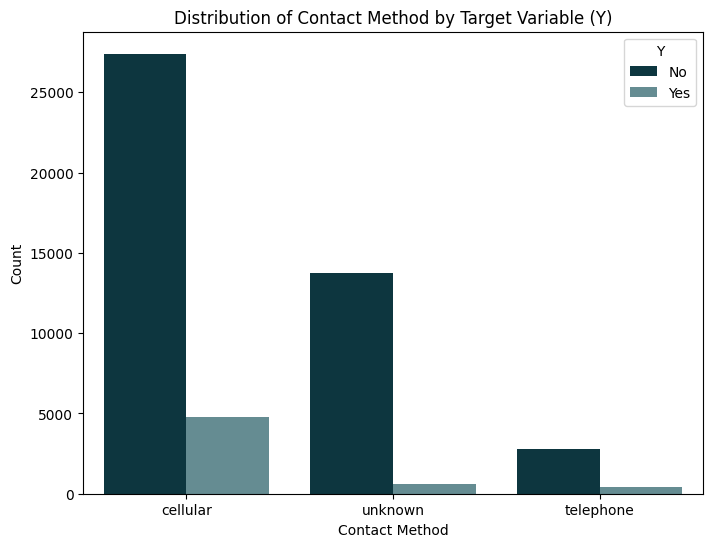
\includegraphics[width=0.7\linewidth]{data/bank_marketing/pic/Bank_Contact.png} \\ \hline
               Month & 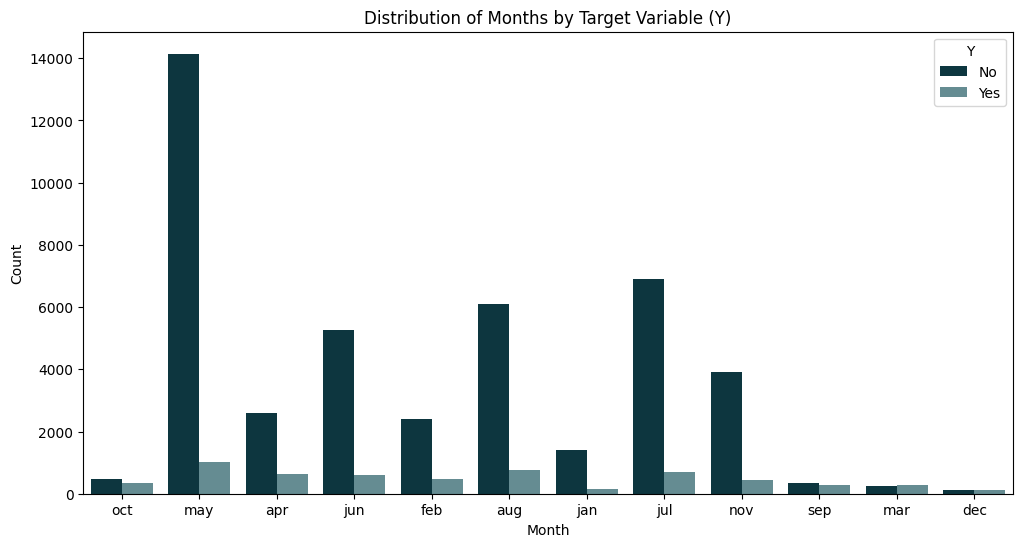
\includegraphics[width=0.7\linewidth]{data/bank_marketing/pic/Bank_Month.png} \\ \hline 
               Poutcome & 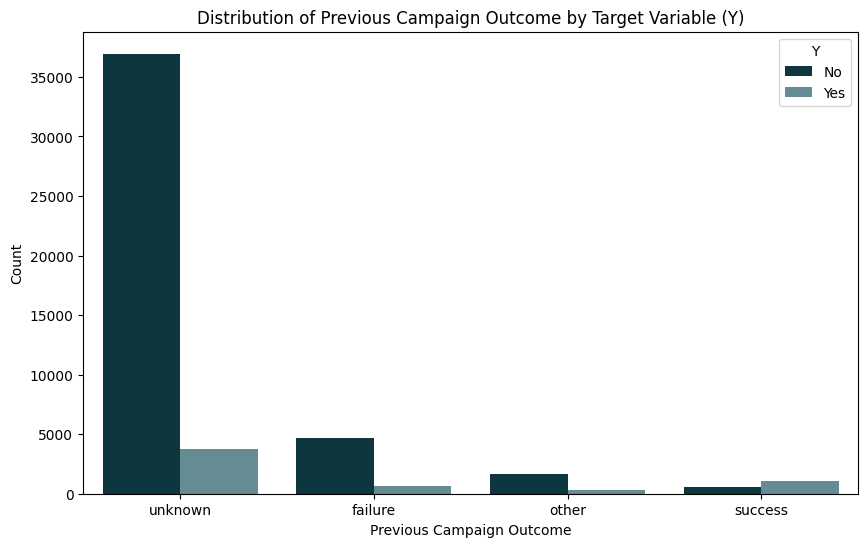
\includegraphics[width=0.7\linewidth]{data/bank_marketing/pic/Bank_Pout.png} \\ \hline
               \hline
               \caption{Distribution of Categorical Variables by Target Variable (Y)}
               \label{tab:attribute_distribution}
           \end{longtable}
           

           \subsubsection{Summary of Categorical Variables (File: Bank\_Add)}

           The provided table (Table \ref{tab:my_label}) furnishes a comprehensive overview of pivotal categorical variables in the dataset. Each row corresponds to a specific attribute, including job type, marital status, education level, default status, housing and loan particulars, contact method, month of contact, day of the week, the outcome of the previous marketing campaign (\textit{Poutcome}), and the target variable '\textit{Y}.' The columns offer crucial insights into the distribution, diversity, and prevalence of these attributes.
           
           \begin{table}[h]
               \centering
               \begin{tabular}{lcccc}
                   \textbf{Attributes} & \textbf{Count} & \textbf{Unique} & \textbf{Top} & \textbf{Freq} \\
                   \hline
                   Job & 45307 & 12 & \textit{admin.} & 11434 \\ 
                   Marital & 45307 & 4 & \textit{married} & 27437 \\ 
                   Education & 45307 & 8 & \textit{university.degree} & 13432 \\ 
                   Default & 45307 & 3 & \textit{no} & 35903 \\ 
                   Housing & 45307 & 3 & \textit{yes} & 23751 \\ 
                   Loan & 45307 & 3 & \textit{no} & 37299 \\ 
                   Contact & 45307 & 2 & \textit{cellular} & 28796 \\ 
                   Month & 45307 & 10 & \textit{May} & 15147 \\ 
                   Day of Week & 45307 & 5 & \textit{Thu} & 9483 \\ 
                   Poutcome & 45307 & 3 & \textit{nonexistent} & 39086 \\ 
                   Y & 45307 & 2 & \textit{no} & 40216 \\ 
               \end{tabular}
               \caption{Summary Statistics of Categorical Variables in the Dataset.}
               \label{tab:my_label}
               \end{table}
           
           \begin{longtable}{|l|c|}
               \hline
               \textbf{Attributes} & \textbf{Distribution Visualization} \\
               \hline
               \endhead
               Job & 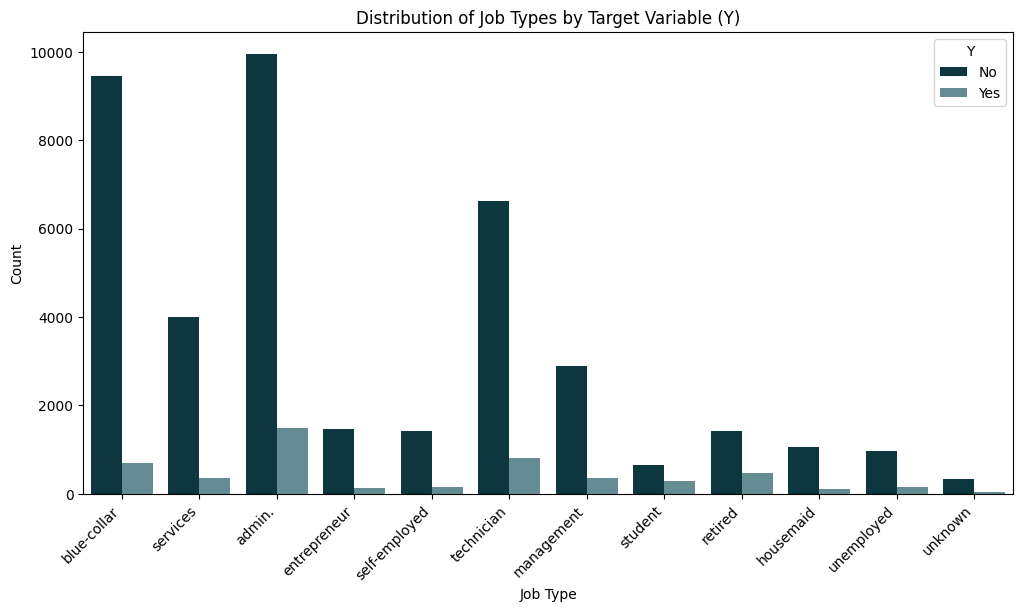
\includegraphics[width=0.7\linewidth]{data/bank_marketing/pic/Bank_Add_job.png} \\ \hline
               Marital & \includegraphics[width=0.7\linewidth]{data/bank_marketing/pic/Bank_Add_marital.png} \\ \hline
               Education & 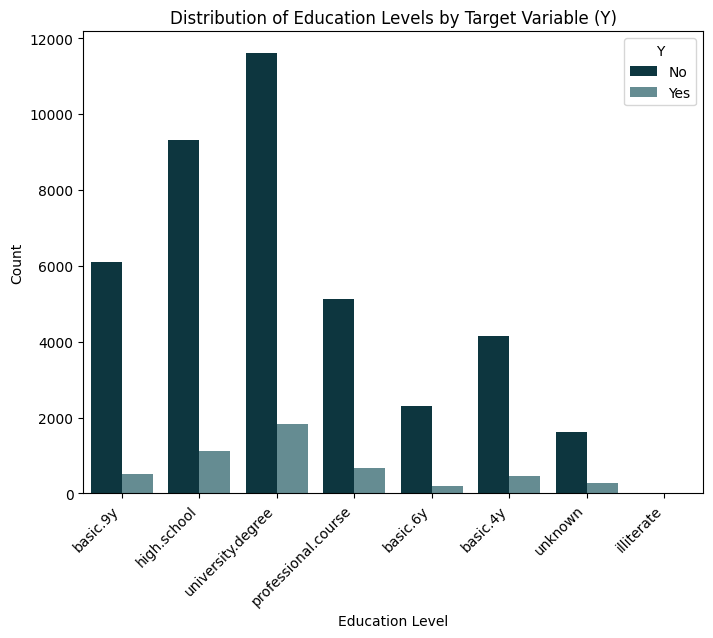
\includegraphics[width=0.7\linewidth]{data/bank_marketing/pic/Bank_Add_edu.png} \\ \hline
               Default & 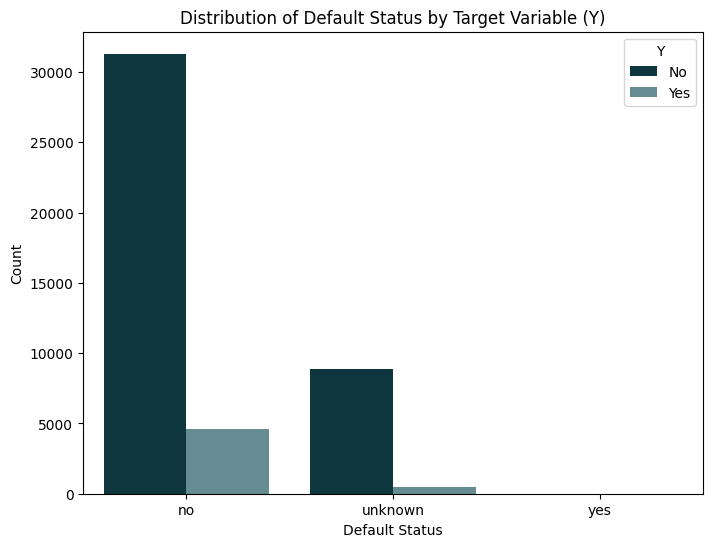
\includegraphics[width=0.7\linewidth]{data/bank_marketing/pic/Bank_Add_def.png} \\ \hline
               Housing & 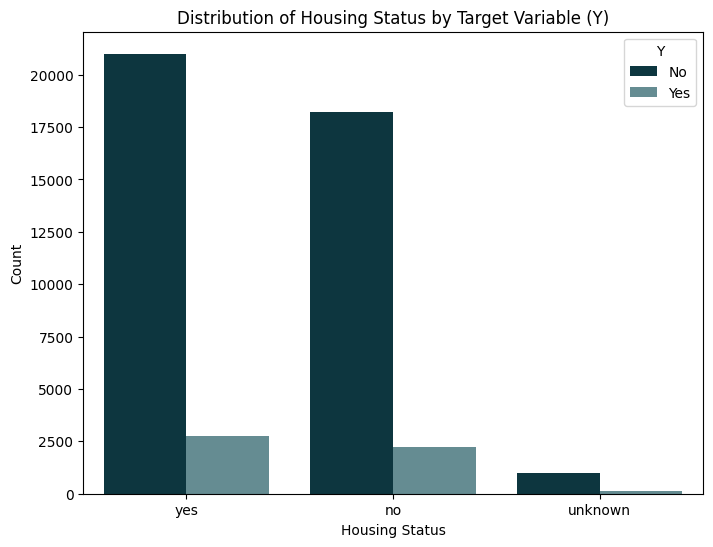
\includegraphics[width=0.7\linewidth]{data/bank_marketing/pic/Bank_Add_Hous.png} \\ \hline
               Loan & 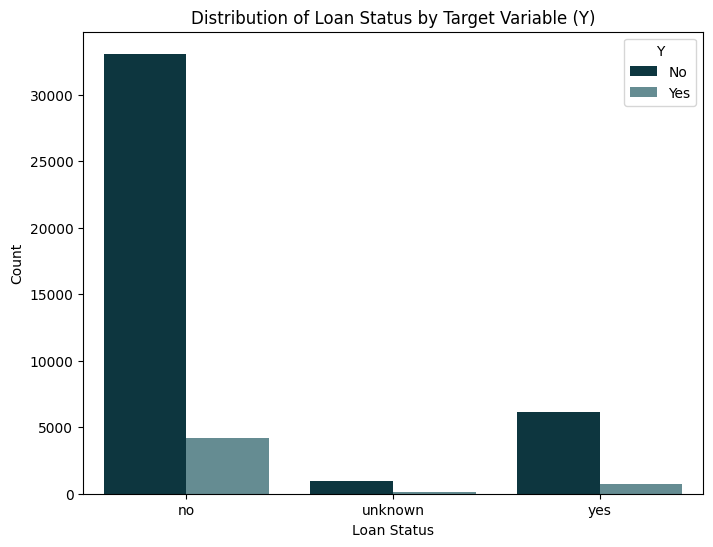
\includegraphics[width=0.7\linewidth]{data/bank_marketing/pic/Bank_Add_loan.png} \\ \hline
               Contact & 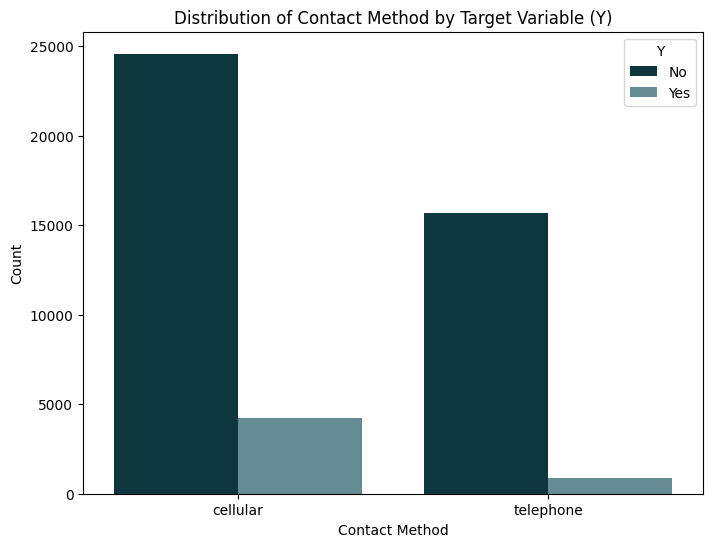
\includegraphics[width=0.7\linewidth]{data/bank_marketing/pic/Bank_Add_Contact.png} \\ \hline
               Month & 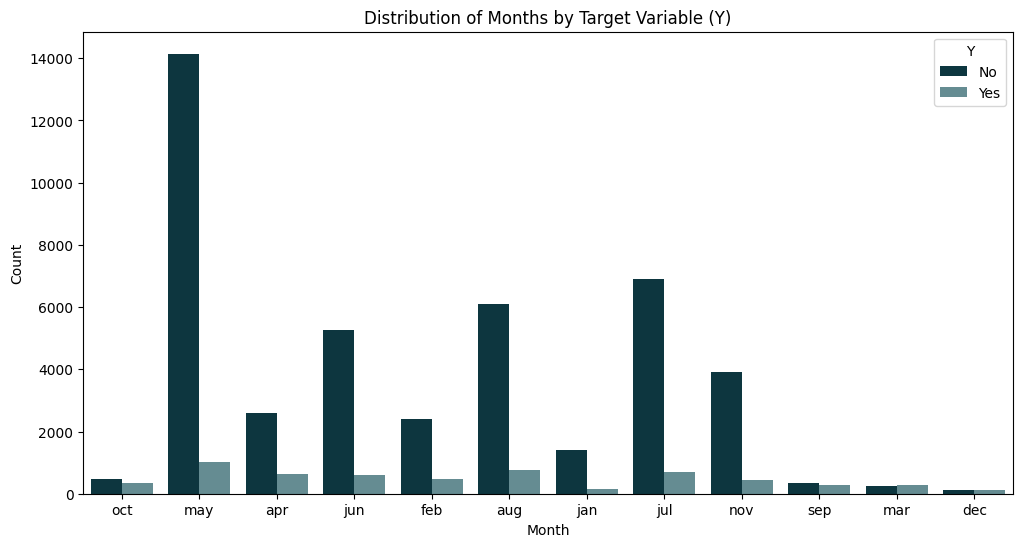
\includegraphics[width=0.7\linewidth]{data/bank_marketing/pic/Bank_Add_Month.png} \\ \hline
               Poutcome & 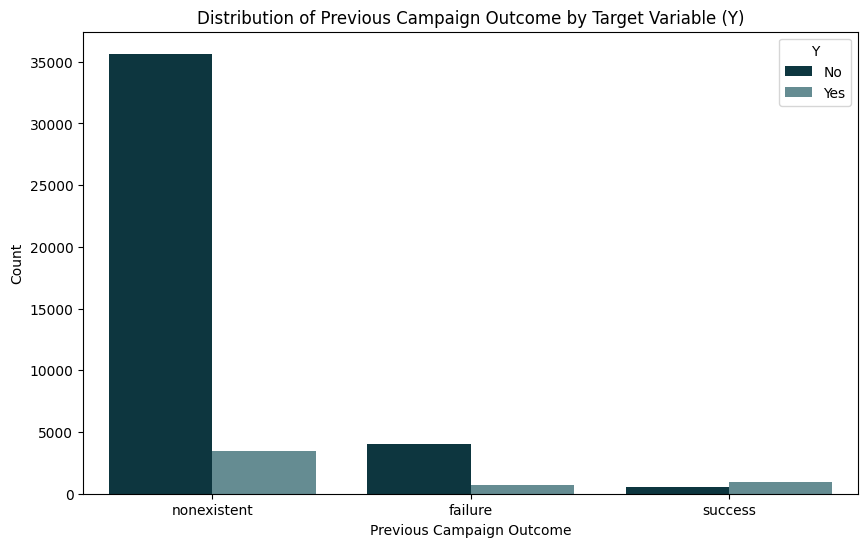
\includegraphics[width=0.7\linewidth]{data/bank_marketing/pic/Bank_Add_Pout.png} \\ \hline
               Day\_Of\_Week & 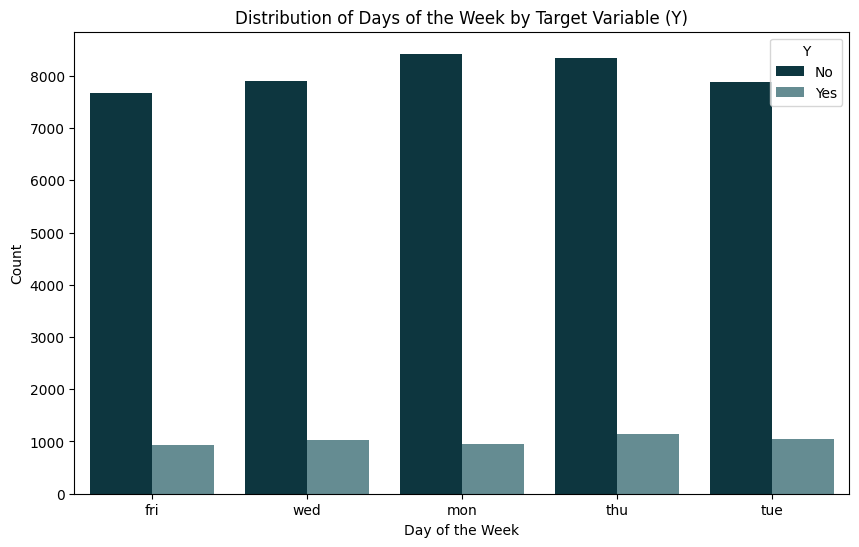
\includegraphics[width=0.7\linewidth]{data/bank_marketing/pic/Bank_Add_Dayweek.png} \\ 
               \hline
               \caption{Distribution of Categorical Variables by Target Variable (Y)}
               \label{tab:attribute_distribution}
           \end{longtable}  


           \subsection{Outlier Detection Process}
           \subsubsection{Introduction to Outliers}
           Outliers in a dataset are data points that deviate significantly from the overall pattern of the data. Identifying and understanding outliers is crucial in data analysis as they can have a substantial impact on statistical measures and influence the interpretation of results. In this chapter, we explore the process of detecting outliers in the \textit{Bank }and \textit{Bank\_Add} datasets, focusing on the application of the Interquartile Range (IQR) and boxplot methods.
           \subsubsection{Interquartile Range (IQR) Method}
           The Interquartile Range (IQR) is a statistical measure that describes the spread of the middle 50\% of the data. To detect outliers using the IQR method, we calculate the IQR by finding the difference between the third quartile (\(Q3\)) and the first quartile (\(Q1\)). Outliers are then identified as data points falling below \(Q1 - 1.5 \times IQR\) or above \(Q3 + 1.5 \times IQR\).
           \subsubsection{Boxplot Visualization}
           A boxplot is a graphical representation that displays the distribution of data and highlights the presence of outliers. The box in the plot represents the interquartile range, with the median marked as a line inside the box. Whiskers extend to the minimum and maximum values within a defined range, and outliers are displayed as individual points beyond the whiskers.
           
           \subsubsection{Outlier Detection (File: Bank)}
           \begin{longtable}{|p{0.15\textwidth}|p{0.18\textwidth}|p{0.17\textwidth}|p{0.40\textwidth}|}
            \caption{Outliers and Boxplots}\label{tab:outliers_boxplots}\\
            \hline
            \textbf{Variable} & \textbf{Statistics} & \textbf{Outliers} & \textbf{Boxplot} \\
            \hline
            \endfirsthead
            \multicolumn{4}{c}%
            {\tablename\ \thetable\ -- \textit{Continued from previous page}} \\
            \hline
            \textbf{Variable} & \textbf{Statistics} & \textbf{Outliers} & \textbf{Boxplot} \\
            \hline
            \endhead
            \hline \multicolumn{4}{r}{\textit{Continued on next page}} \\
            \endfoot
            \hline
            \endlastfoot
        
            \textbf{Age} & 
            \begin{itemize}
                \item 541 outliers
                \item Min: 71.0
                \item Max: 95.0
                \item Mean: 76.8
                \item Std: 4.74
            \end{itemize} & 
            \begin{itemize}
                \item $Q1$ : 33
                \item $Q3$ : 48
                \item $IQR$ : 15.0
            \end{itemize} &
            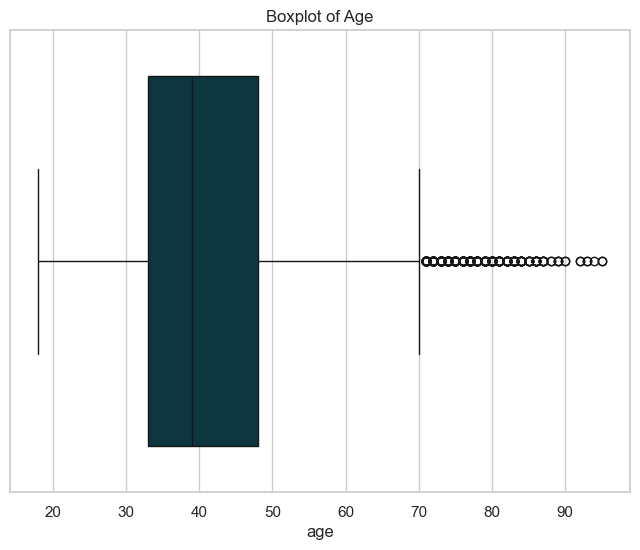
\includegraphics[width=0.40\textwidth]{data/bank_marketing/pic/Outlier/Age.png} \\
            \hline
            \textbf{Balance} & 
            \begin{itemize}
                \item 5237 outliers
                \item Min: -8019.0
                \item Max: 102127.0
                \item Mean: 7544.1
                \item Std: 6255.82
            \end{itemize} & 
            \begin{itemize}
                \item $Q1$ : 72
                \item $Q3$ : 1431
                \item $IQR$ : 1359
            \end{itemize} &
            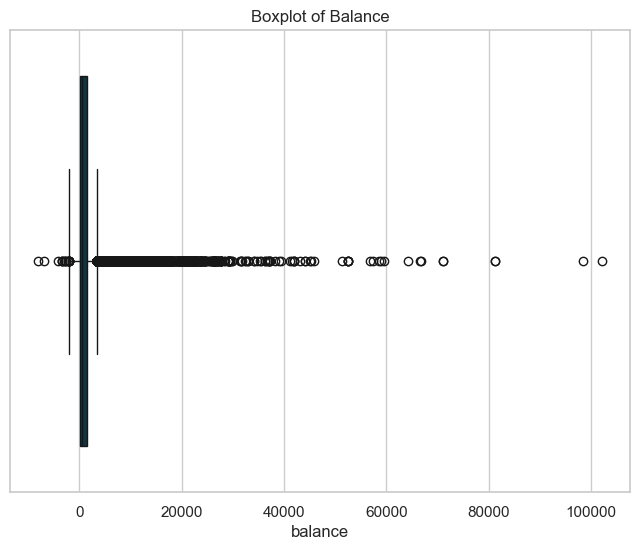
\includegraphics[width=0.40\textwidth]{data/bank_marketing/pic/Outlier/balance.png} \\
            \hline
            \textbf{Day} & 
            \begin{itemize}
                \item 0 outliers
                \item Min: nan
                \item Max: nan
                \item Mean: nan
                \item Std: nan
            \end{itemize} & 
            \begin{itemize}
                \item $Q1$ : 8
                \item $Q3$ : 21
                \item $IQR$ : 13
            \end{itemize} &
            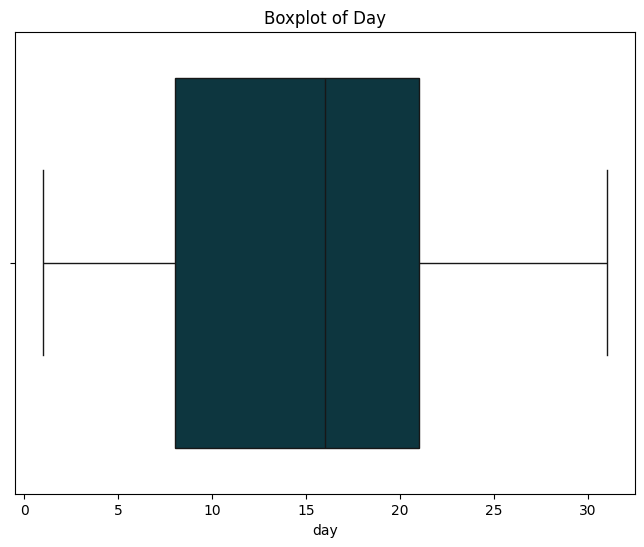
\includegraphics[width=0.40\textwidth]{data/bank_marketing/pic/Outlier/Day.png} \\
            \hline
            \textbf{Duration} & 
            \begin{itemize}
                \item 3566 outliers
                \item Min: 646.0
                \item Max: 4918.0
                \item Mean: 967.81
                \item Std: 354.91
            \end{itemize} & 
            \begin{itemize}
                \item $Q1$ : 103
                \item $Q3$ : 320
                \item $IQR$ : 217
            \end{itemize} &
            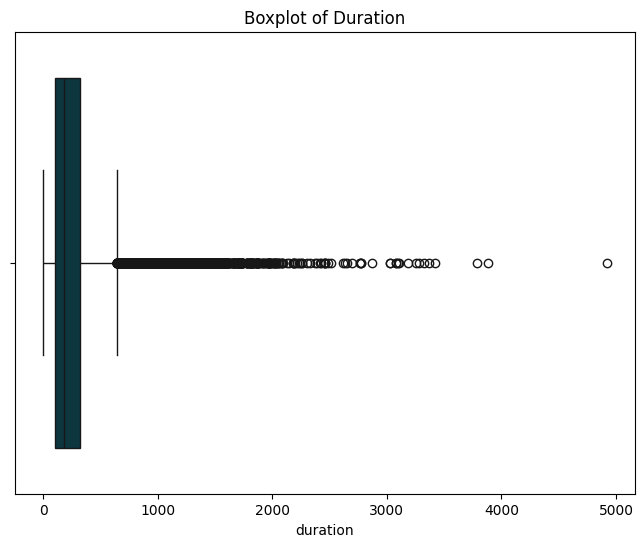
\includegraphics[width=0.40\textwidth]{data/bank_marketing/pic/Outlier/Duration.png} \\
            \hline
            \textbf{Campaign} & 
            \begin{itemize}
                \item 3382 outliers
                \item Min: 7.0
                \item Max: 63.0
                \item Mean: 11.48
                \item Std: 6.0
            \end{itemize} & 
            \begin{itemize}
                \item $Q1$ : 1
                \item $Q3$ : 3
                \item $IQR$ : 2
            \end{itemize} &
            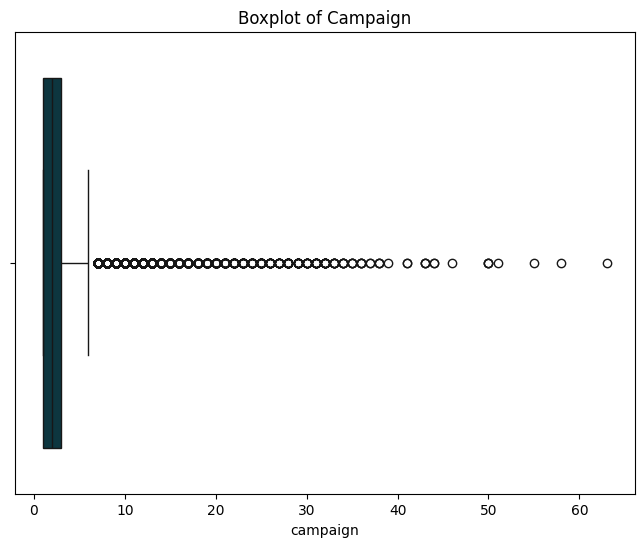
\includegraphics[width=0.40\textwidth]{data/bank_marketing/pic/Outlier/Campaign.png} \\
            \hline
            \textbf{Pdays} & 
            \begin{itemize}
                \item 9073 outliers
                \item Min: 1.0
                \item Max: 871.0
                \item Mean: 224.6
                \item Std: 115.5
            \end{itemize} & 
            \begin{itemize}
                \item $Q1$ : -1
                \item $Q3$ : -1
                \item $IQR$ : 0
            \end{itemize} &
            \includegraphics[width=0.40\textwidth]{data/bank_marketing/pic/Outlier/Pdays.png} \\
            \hline
            \textbf{Previous} & 
            \begin{itemize}
                \item 9073 outliers
                \item Min: 1.0
                \item Max: 275.0
                \item Mean: 3.16
                \item Std: 4.43
            \end{itemize} & 
            \begin{itemize}
                \item $Q1$ : 0
                \item $Q3$ : 0
                \item $IQR$ : 0
            \end{itemize} &
            \includegraphics[width=0.40\textwidth]{data/bank_marketing/pic/Outlier/Previous.png} \\
            \hline
        \end{longtable}
           
        \vspace{100pt}
           
           \subsubsection{Outlier Detection (File: Bank\_Add)}
           
           \begin{longtable}{|p{0.15\textwidth}|p{0.18\textwidth}|p{0.17\textwidth}|p{0.40\textwidth}|}
            \caption{Outliers and Boxplots}\label{tab:outliers_boxplots}\\
            \hline
            \textbf{Variable} & \textbf{Statistics} & \textbf{Outliers} & \textbf{Boxplot} \\
            \hline
            \endfirsthead
            \multicolumn{4}{c}%
            {\tablename\ \thetable\ -- \textit{Continued from previous page}} \\
            \hline
            \textbf{Variable} & \textbf{Statistics} & \textbf{Outliers} & \textbf{Boxplot} \\
            \hline
            \endhead
            \hline \multicolumn{4}{r}{\textit{Continued on next page}} \\
            \endfoot
            \hline
            \endlastfoot
            
            \textbf{Age} & 
            \begin{itemize}
                \item 508 outliers
                \item Min: 70.0
                \item Max: 98.0
                \item Mean: 76.915
                \item Std: 5.7
            \end{itemize} & 
            \begin{itemize}
                \item $Q1$ : 32
                \item $Q3$ : 47
                \item $IQR$ : 15.0
            \end{itemize} &
            \includegraphics[width=0.40\textwidth]{data/bank_marketing/pic/Outlier/Age_Add.png} \\
            \hline
            \textbf{Duration} & 
            \begin{itemize}
                \item 3249 outliers
                \item Min: 645.0
                \item Max: 4918.0
                \item Mean: 967.69
                \item Std: 367.12
            \end{itemize} & 
            \begin{itemize}
                \item $Q1$ : 102
                \item $Q3$ : 319
                \item $IQR$ : 217
            \end{itemize} &
            \includegraphics[width=0.40\textwidth]{data/bank_marketing/pic/Outlier/Duration_Add.png} \\
            \hline
            \textbf{Campaign} & 
            \begin{itemize}
                \item 2641 outliers
                \item Min: 7.0
                \item Max: 56.0
                \item Mean: 11
                \item Std: 5.33
            \end{itemize} & 
            \begin{itemize}
                \item $Q1$ : 1
                \item $Q3$ : 3
                \item $IQR$ : 2
            \end{itemize} &
            \includegraphics[width=0.40\textwidth]{data/bank_marketing/pic/Outlier/Campaign_Add.png} \\
            \hline
            \textbf{Pdays} & 
            \begin{itemize}
                \item 1675 outliers
                \item Min: 0.0
                \item Max: 27.0
                \item Mean: 6.0
                \item Std: 3.83
            \end{itemize} & 
            \begin{itemize}
                \item $Q1$ : 999.0
                \item $Q3$ : 999.0
                \item $IQR$ : 0
            \end{itemize} &
            \includegraphics[width=0.40\textwidth]{data/bank_marketing/pic/Outlier/Pdays_Add.png} \\
            \hline
            \textbf{Previous} & 
            \begin{itemize}
                \item 6221 outliers
                \item Min: 1.0
                \item Max: 7
                \item Mean: 1.27
                \item Std: 0.65
            \end{itemize} & 
            \begin{itemize}
                \item $Q1$ : 0
                \item $Q3$ : 0
                \item $IQR$ : 0
            \end{itemize} &
            \includegraphics[width=0.40\textwidth]{data/bank_marketing/pic/Outlier/Previous_Add.png} \\
            \hline
            \textbf{Employment Variation Rate} & 
            \begin{itemize}
                \item 0 outliers
                \item Min: nan
                \item Max: nan
                \item Mean: nan
                \item Std: nan
            \end{itemize} & 
            \begin{itemize}
                \item $Q1$ : -1.8
                \item $Q3$ : 1.4
                \item $IQR$ : 3.2
            \end{itemize} &
            \includegraphics[width=0.40\textwidth]{data/bank_marketing/pic/Outlier/Emp.png} \\
            \hline
            \textbf{Consumer Price Index} & 
            \begin{itemize}
                \item 0 outliers
                \item Min: nan
                \item Max: nan
                \item Mean: nan
                \item Std: nan
            \end{itemize} & 
            \begin{itemize}
                \item $Q1$ : 93.075
                \item $Q3$ : 93.994
                \item $IQR$ : 0.91
            \end{itemize} &
            \includegraphics[width=0.40\textwidth]{data/bank_marketing/pic/Outlier/price.png} \\
            \hline
            \textbf{Consumer Confidence Index} & 
            \begin{itemize}
                \item 490 outliers
                \item Min: -26.9
                \item Max: -26.9
                \item Mean: -26.99
                \item Std: 7.11
            \end{itemize} & 
            \begin{itemize}
                \item $Q1$ : -42.7
                \item $Q3$ : -36.4
                \item $IQR$ : 6.33
            \end{itemize} &
            \includegraphics[width=0.40\textwidth]{data/bank_marketing/pic/Outlier/conf.png} \\
            \hline
            \textbf{EURIBOR 3-Month Rate} & 
            \begin{itemize}
                \item 0 outliers
                \item Min: nan
                \item Max: nan
                \item Mean: nan
                \item Std: nan
            \end{itemize} & 
            \begin{itemize}
                \item $Q1$ : 1.344
                \item $Q3$ : 4.961
                \item $IQR$ : 3.617
            \end{itemize} &
            \includegraphics[width=0.40\textwidth]{data/bank_marketing/pic/Outlier/Eur.png} \\
            \hline
            \textbf{Number of Employees} & 
            \begin{itemize}
                \item 0 outliers
                \item Min: nan
                \item Max: nan
                \item Mean: nan
                \item Std: nan
            \end{itemize} & 
            \begin{itemize}
                \item $Q1$ : 5099.1
                \item $Q3$ : 5228.1
                \item $IQR$ : 129.0
            \end{itemize} &
            \includegraphics[width=0.40\textwidth]{data/bank_marketing/pic/Outlier/num.png} \\
            \hline
            \end{longtable}

            In conclusion, the Exploratory Data Analysis (EDA) chapter plays a pivotal role in our report, serving as the foundation for understanding and interpreting the dataset under investigation. Through a systematic and comprehensive exploration of the data, we have gained valuable insights into its characteristics, distribution, and potential patterns. The visualizations and statistical summaries presented in this chapter have not only facilitated a clearer understanding of the dataset but have also laid the groundwork for subsequent analyses.

            EDA has allowed us to identify key trends, outliers, and relationships within the data, providing a basis for informed decision-making in later stages of our study. Moreover, the exploratory phase has highlighted potential areas for further investigation and hypothesis testing. By uncovering patterns and correlations, EDA aids in generating hypotheses that can be tested through more advanced statistical methods.
            
            The visual representations, such as histograms, scatter plots, and box plots, have proven to be effective tools for conveying complex information in a comprehensible manner. These visuals enhance the interpretability of the data, making it more accessible to a wider audience.
            
            In summary, the EDA chapter is a crucial step in the data analysis process, acting as a bridge between raw data and meaningful insights. The patterns and trends discovered during this phase serve as a solid foundation for subsequent analyses, ensuring that our conclusions and recommendations are rooted in a thorough understanding of the dataset. Through the lens of EDA, we have not only explored the data but have paved the way for deeper investigations and a more nuanced interpretation of our research findings.


            
\section{Data Refinement: Preprocessing Strategies for Enhanced Analysis}

\subsection{Handling Outliers: Binning, Winsorizing, and Log Transformation}
In the exploration of our dataset, robust strategies were employed to identify and handle outliers, ensuring the integrity of subsequent analyses. The following methods, namely Binning, Winsorizing, and Log Transformation, were judiciously applied to manage extreme values.

\subsubsection{Binning: Age Categorization for Improved Interpretation}

Recognizing the importance of age in our analysis, a binning technique was employed to categorize ages into groups. This not only enhances the interpretability of age-related insights but also provides a structured framework for managing potential outliers within specific age ranges.

\subsubsection{Log Transformation: Addressing Right-Skewed Distributions}
For variables like \textit{balance} a log transformation was applied to mitigate the impact of right-skewed distributions. This transformation not only reduces the influence of outliers but also provides a more symmetric representation of the data.

\subsubsection{Managing Outliers: Winsorizing with Log Transformation}
\textbf{Winsorizing}
Extreme values in \textit{duration}, \textit{campaign} , \textit{pdays}, \textit{previous}, and \textit{Consumer Confidence Index}  were identified and capped using the Winsorizing technique. This involved replacing values beyond the 5th and 95th percentiles with less extreme values, effectively mitigating the impact of outliers.

\textbf{Log Transformation}
Following Winsorizing, a log transformation was applied to the variables \textit{duration}, \textit{campaign} , \textit{pdays}, \textit{previous}, and \textit{Consumer Confidence Index} . This step is instrumental in reducing the influence of extreme values, ensuring a more normalized distribution for these variables.
\\
\\
By adopting this combined approach of Winsorizing and Log Transformation, we strike a balance between preserving the integrity of the data and managing the impact of extreme values. These steps contribute to a more reliable dataset, ensuring the stability and accuracy of subsequent analyses.

\subsection{Label Encoding for Categorical Variables}
Categorical variables, such as \textit{job} ,\textit{age} \textit{marital}, \textit{education}, \textit{default}, \textit{housing}, \textit{loan}, \textit{contact}, \textit{month}, and \textit{poutcome}, were present in the dataset. As machine learning models require numerical input, these categorical variables were subjected to label encoding.

Label encoding involves assigning a unique numerical code to each category within a variable. This transformation allows for the representation of categorical data in a format suitable for mathematical modeling.

The textit{LabelEncoder} class from the textit{scikit-learn} library was employed for this task. Each category within the categorical variables was assigned a unique numerical code based on its order of appearance in the dataset.
\\
The label encoding was applied to the following columns:
\begin{itemize}
    \item age
    \item marital
    \item education
    \item job
    \item default
    \item housing
    \item loan
    \item contact
    \item month
    \item poutcome
\end{itemize}

The encoded columns were added to the dataset with the suffix \textit{\_encoded} , providing a numerical representation of the original categorical data.
The encoded dataset serves as the input for subsequent machine learning tasks.

\subsection{ Dimensionality Reduction with Principal Component Analysis (PCA)}

In this section, we explore the application of Principal Component Analysis (PCA) to reduce the dimensionality of our datasets, namely the primary banking dataset textit{Bank} and its supplementary dataset textit{Bank\_Add}. The primary goal is to distill the information within the datasets while maintaining their essential characteristics.

\subsubsection{ Data Preparation}
We commence by preparing the datasets, extracting the features and target variables for both textit{Bank} and textit{Bank\_Add}.
\subsubsection{Standardization}
To ensure that all features contribute uniformly to the principal components, we employ a standardization process. This step is crucial for eliminating scale-based biases in the dataset.
\subsubsection{Principal Component Analysis (PCA)}
Applying PCA to the standardized datasets allows us to transform the original features into a set of principal components. The number of components retained is a critical decision point and is often determined by the desired level of explained variance.
\subsubsection{Explained Variance Analysis}
We delve into the analysis of the explained variance ratio to gain insights into the information retained by each principal component. This step aids in determining the appropriate number of components to retain for subsequent analyses.
\subsubsection{Visualizations}
Visual representations provide a more intuitive understanding of the results. A plot depicting the cumulative explained variance facilitates the identification of an optimal number of components to retain. Additionally, scatter plots in the reduced feature space allow for a visual examination of the distribution of data points.
\subsubsection{Findings}
The application of PCA has yielded a reduced-dimensional representation of the datasets, encapsulating a substantial portion of the original information. The visualizations offer insights into the grouping of data points in the reduced feature space, paving the way for more streamlined analyses and machine learning applications.










\end{document}



